\section{Il piede torto}

Nell'ambito delle patologie del piede, possiamo considerare il piede normale al centro di una fascia e agli estremi di questa troviamo:

\begin{itemize}
\item
  Nell'ambito \textbf{\emph{dell'eccesso di pronazione}}, il \emph{piede torto congenito astragalo-verticale} o ``a dondolo'': forma più grave dal punto di vista clinico perché congenito.
\emph{Oltre a questa}, ci sono \emph{le forme di piede piatto} che abbiamo visto: piede piatto da acinostosi, piede piatto essenziale.
\item
  Dall'altra parte, come \textbf{\emph{eccesso di supinazione}}, il \emph{piede torto equino varo supinato} come forma più grave. \emph{Questa denominazione (equino-varo-supinato) indica la coesistenza di tre componenti:}

\begin{itemize}
\item
  \emph{Equinismo}
\item
  \emph{Varismo}
\item
  \emph{Supinazione}
\end{itemize}

Sarà chiaro nella parte che segue come queste tre componenti si associno nella manifestazione clinica di questa deformità.

Tra il piede normale e il piede torto equino varo supinato (ai due estremi) ci sono tutte le altre forme in eccesso di supinazione
\end{itemize}

\emph{Da quanto detto risulta fin da subito chiaro che piede torto non significa solo piede equino-varo-supinato perché ci sono molte altre forme di piede torto oltre questa:}

\begin{itemize}
\item
  \emph{L' astragalo-verticale}
\item
  \emph{Il talo valgo pronato}
\item
  \emph{L'avampiede addotto}
\item
  \emph{Il metatarso varo}
\end{itemize}

\emph{Da ricordare: Ha durante lo sviluppo fetale è normale che il feto abbia ad un certo punto il piede equino varo supinato... poi piano fino alla nascita c'è una desupinazione e fino a 4 anni di età c'è un eccesso di pronazione. Quindi, ci sono delle fasi di alternanza di supinazione e pronazione. Poi da 4 anni in su con gli stimoli esterni, si va verso il piede normale, ecco perché prima dei 4 anni non si parla di piede piatto.}

\subsection{Piede torto congenito}

\textbf{Congenito} significa \emph{connatale} ovvero presente alla nascita e può essere ereditario o meno. Dunque connatale non vuol dire \emph{ereditario}: il concetto di ereditarietà è legato alla consapevolezza o meno che certi geni determino quel fenotipo (in questo caso quella deformità). Nelle forme ereditarie saranno coinvolti e caratterizzati dei cromosomi che determinano una certa situazione rispondente a sua volta alle leggi di Mendel - quindi a un modello di tipo matematico. \emph{Un qualcosa di genetico potrebbe anche presentarsi alla nascita quindi essere anche connatale oppure presentarsi più avanti nella vita}. Connatale non vuol dire nemmeno
\emph{familiare}: una famiglia può avere il piede torto e un'altra no; quel gruppo famigliare può aver avuto delle influenze rispetto all'altra. Entrano in gioco anche delle predisposizioni ereditarie, ma anche delle influenze esterne a cui quel gruppo familiare viene sottoposto.

\subsubsection{Definizione}

\textbf{Il piede torto congenito è una deformità presente alla nascita (connatale) caratterizzata dall'alterazione permanente della morfologia del piede e dei suoi rapporti con la gamba}. Questo concetto è particolarmente importante perché nel caso del piede torto, ci si
potrebbe aspettare solo una deformità a livello del piede invece non è così! Chi è affetto da piede torto ad esempio, presenta una \emph{ipomiotrofia} dei muscoli della sura: il polpaccio appare molto più piccolo, è detto polpaccio ad imbuto. Si tratta di una situazione
non recuperabile anche se quell'individuo cominciasse ad allenarsi nel tentativo di sviluppare quel muscolo e non riuscirebbe proprio perché c'è una patologia congenita a livello di tutto l'arto.
\emph{\textbf{Quindi si tratta di una malattia di tutto l'arto inferiore \emph{la cui estrinsecazione clinica è prevalentemente a livello del piede.}} }

La definizione va completa perché nel piede torto congenito c'è anche un'\textbf{alterazione dei rapporti tra il retropiede e l'avampiede}.

\emph{Inoltre è necessario tener conto del fatto che spesso una malformazione può nascondere altre malformazioni: il piede torto potrebbe essere un campanello d'allarme per altre malformazioni per
esempio una displasia congenita dell'anca. Sulla base di ciò è sempre consigliato in un bambino con piede torto eseguire una radiografia a quattro mesi per controllare la presenza di displasia congenita dell'anca. Solitamente c'è un'alta percentuale di malformazioni ulteriori nei bambini affetti da piede torto sia a livello ortopedico che in altri distretti.}

\emph{Il concetto appena esposto dovrebbe esser sempre mantenuto di fronte ad ogni deformità perché ci permetterebbe di diagnosticare precocemente situazioni patognomoniche che magari si estrinsecherebbero più avanti con l'età: una malformazione anche piccola come la sindattilia (dita del piede e della mano fuse) potrebbe nascondere una displasia congenita dell'anca o un `altra malformazione o peggio essere l'estrinsecazione di una patologia sistemica.}

\emph{Sarebbe a questo punto molto importante differenziare tra il piede torto congenito \emph{isolato}, cioè che si presenza da solo, senza altre deformità congenite ed il piede torto congenito inserito in una
\emph{sindrome generale} come l'artrogriposi. Infatti non è raro riscontrare questa condizione in associazione con altre deformità quali la displasia dell'anca o le rigidità articolari congenite multiple. Tale distinzione ha anche un notevole impatto prognostico perché le forme di piede torto isolato sono in genere più facilmente correggibili rispetto a quelle associate ad altre deformità}

\emph{Nel caso invece di un piede torto in una persona con alterazioni a livello del sistema nervoso periferico, se curassimo la malformazione del piede, queste persone non potrebbero comunque camminare ergo non ne varrebbe la pena. Questo è importante nella scelta del trattamento
perché non bisogna fare interventi dolorosi su pazienti che presentano problematiche che comunque non gli permetteranno di camminare.}

\subsubsection{Epidemiologia }

Ha una frequenza di 1 caso su 1000 nati: rara, ma comunque presente. \emph{È tra le deformità congenite di interesse ortopedico la seconda più comune dopo la displasia congenita dell'anca. Talvolta è possibile evidenziare un certo grado di \emph{familiarità} per questa patologia che depone a favore di una certa suscettibilità genetica ed i maschi risultano peraltro più colpiti che le femmine con un rapporto di 2 a 1.}

\emph{N.B. E' importante tenere a mente il rapporto di incidenza nei due sessi, ma non bisogna escludere mai a priori la possibilità di comparsa
anche nel sesso meno coinvolto.}

\subsubsection{Forme cliniche}

Sono sostanzialmente quattro:

\begin{itemize}
\item[1.]
  \emph{\textbf{Equino} \textbf{cavo varo supinato}} (il cavismo è una componente del piede in eccesso di supinazione). Rappresenta circa il 65\% dei casi di piede torto
\item[2.]
  \textbf{\emph{Talo valgo pronato}}: il 20\% dei casi
\item[3.]
  \textbf{\emph{Metatarso varo}}: il 10\% dei casi
\item[4.]
  \textbf{\emph{Valgo convesso o astragalo verticale o \emph{piede reflesso} o piede a dondolo}:} si tratta del 5\% dei casi però è il più grave
\end{itemize}

Può essere sia \textbf{monolaterale} (50\%) che \textbf{bilaterale} (50\%) \emph{anzi queste ultime forme sono di pochissimo più comuni rispetto a quelle monolaterali.}

Ci sono:

\begin{itemize}
\item
  Forme che si manifestano nell'ambito di gravi sindromi come ad es. l'artrogriposi che portano a morte o a delle invalidità che non sono legate solo ed esclusivamente al piede torto
\item
  Forme sporadiche (isolate) in cui il bambino non mostra alcuna alterazione funzionale però presenta uno od entrambi i piedi torti.
\end{itemize}

Questi sono un po' i due casi estremi con le varie variabili interposte.

Bisogna distinguere fin da subito tra \emph{normalità} \emph{anatomica} (piede normale) e \emph{normalità della vita} (vita normale).

Es. una persona che porta gli occhiali è un invalido, ma portandoli conduce una vita normale.

Nelle forme sporadiche dove è presente solamente il piede torto e \emph{non c'è nessuna alterazione funzionale}, è importante far capire ai genitori che vi è la possibilità di condurre una vita normale pur se il piede e non è ``normale'' morfologicamente. Si tratta di un concetto
fondamentale nell'ambito dell'ortopedia e della traumatologia. Ci sono persone che conducono una vita assolutamente normale pur col piede torto (calciatori, chirurghi) e questo perché non c'è un'alterazione
funzionale.

Inoltre è sempre bene valutare anche la componente psichica che impatterà sul successo del percorso terapeutico eventualmente intrapreso: il malformato congenito in genere è più accomodante rispetto al paziente con malformazione acquisito (ad esempio poliomielitico) che tendenzialmente non è mai soddisfatto dell'esito del trattamento.

\subsubsection{Eziopatogenesi}

Si parla di eziologia multifattoriale e s\emph{ono state fatte formulate diverse ipotesi per giustificarne lo sviluppo del piede torto:}

\begin{itemize}
\item
  \textbf{Teoria genetica}. \emph{La teoria genetica considera la possibilità di un gene difettoso che può causare questa malformazione. Questa situazione è particolarmente grave perché nonostante le cure, il piede torto tende a recidivare e tornare nella sua posizione errata. Le forme genetiche nella pratica si riescono a riconoscere perché ci si trova di fronte piedi molto più rigidi e meno riducibili.} \emph{A favore di questa teoria il fatto che essa possa giustifica la possibile suscettibilità familiare di questa patologia e anche la particolare gravità di alcune forme che tendono a recidivare anche dopo correzioni ripetute.}
\item
  \textbf{Teoria meccanica}: oligoidramnios (poco liquido amniotico) o gravidanze gemellari che portano a mantenere il piede in una certa posizione. \emph{Quando c'è poco liquido amniotico o quando ci sono due gemelli, si sviluppa una compressione sulla struttura del piede in via di sviluppo che nasce quindi deformato. Questa teoria è oggi ritenuta valida soprattutto per le forme più lievi e benigne di piede torto congenito che sono considerate benigne perché sono date da posizione (in ortopedia non bisogna mai parlare di postura) errata e non da un codice genetico errato. Si tratta di forme che migliorerebbero anche da sole, ma che vengono comunque trattate e danno buoni risultati.}
\item
  \textbf{Teoria neuromuscolare}\emph{. Era invece piuttosto in voga alcuni anni fa e poneva l'attenzione su di un'alterata attività della placca neuromuscolare. A seguito di questa alterata attività si avrebbe un'ipotrofia primitiva dei muscoli della gamba i quali non sarebbero quindi in grado di compensarsi reciprocamente in modo adeguato e indurrebbero pertanto un'alterazione dei rapporti anatomici tra le ossa del piede su cui vanno ad inserirsi.}
\item
  \textbf{Teoria dell'arresto di sviluppo intrauterino}: a oggi la più accreditata. Nell'ambito della 8a-10a settimana il piede è in equino varo supinazione quindi se c'è un arresto di sviluppo, per qualunque causa, il piede rimarrà in questo stato.
\end{itemize}

\emph{Ad ogni modo, nessuna di queste teorie è riuscita sinora a prevalere nettamente sulle altre anche perché in realtà \emph{non si escludono a vicenda}, sebbene negli ultimi anni si tenda a dare più importanza all'ipotesi del mancato sviluppo intrauterino, anche le altre teorie restano valide, e quello che conta è tenere sempre a mente che di fronte al reperto obiettivo (cioè la presenza del piede torto congenito) è molto importante cercare di identificarne la causa precisa in quanto a seconda del fattore eziologico di base \emph{varia anche la prognosi}
(migliore per le forme di oligoidramnios, peggiore per le forme genetiche).}

Probabilmente non esiste il piede torto, ma ne esistono diverse forme in funzione della eziopatogenesi e ognuno di questi avrà una diversa prognosi.

\subsubsection{Prognosi}

Distinguiamo i vari casi:

\begin{itemize}
\item
  \textbf{Genetico}: ha la prognosi peggiore e dà più problemi: il piede è più duro e va seguito fino alla fine dell'accrescimento
\item
  \textbf{Meccanico} ha una prognosi generalmente buona infatti possono guarire anche spontaneamente. In questo caso i piedi sono più morbidi e più elastici
\item
  \textbf{Neuromuscolare:} prognosi variabile
\end{itemize}

\textbf{NB: C'è un rapporto tra l'eziologia (le 4 teorie), la riducibilità e la prognosi}.
\\\\
Ecografia 3D ed Ecografia tradizionale

\begin{figure}[!ht]
\centering
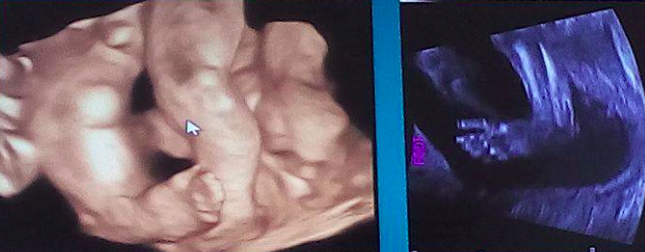
\includegraphics[width=0.4\textwidth]{016/image1.png}
\end{figure}

Quando c'è questo \textbf{dermatoglifo} (freccia) di solito si tratta di un piede torto congenito genetico che è molto rigido.

\begin{figure}[!ht]
\centering
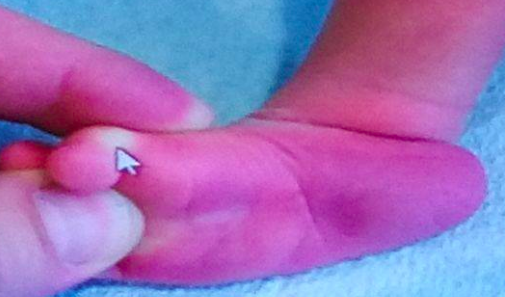
\includegraphics[width=0.4\textwidth]{016/image2.png}
\end{figure}

Nel tentativo di ridurre la rigidità (viene applicata una certa forza) c'è un'ischemia sia dell'alluce del neonato sia del dito dell'esaminatore. Quindi un dermatoglifo così profondo è la firma o segno inconfondibile del piede torto congenito.

\subsubsection{Deformità associate}

La malformazione può essere leggera o grave. Alcune malformazioni sono visibili, altre no (es. displasia congenita dell'anca). Quindi, all'atto del primo esame, se c'è un piede torto, bisogna avere il sospetto che ci siano deformità associate (anche più gravi).

Figura 1: radiografia di un bambino di 4 mesi con segni tipici di \textbf{displasia congenita dell'anca}; si può notare:

\begin{itemize}
\item
  \emph{La sfuggenza del tetto acetabolare (sporge oltre i 35 gradi)}
\item
  Ipoplasia/ritardo nella comparsa del nucleo cefalico femorale (che compare normalmente intorno al sesto mese di vita)
\item
  \emph{Interruzione dell'ogiva di Shenton (arco formato dal margine inferiore della metafisi femorale e dal margine inferiore della branca ileo-pubica)}
\end{itemize}

Questa è nota come triade di Putti: serie di alterazione radiografiche che permettono la diagnosi di displasia congenita dell'anca.
\emph{Bisognerebbe eseguire una Rx a 4 mesi anche se oggi c'è a disposizione anche l'ecografia che permette una diagnosi ancor più precoce.}

\emph{N.B. Un'ecografia normale dell'anca alla nascita non esclude la deformità infatti la displasia congenita dell'anca è un alterazione dello sviluppo quindi è consigliato farne 2/3 nei primi mesi di vita. Se si osserva un'alterazione con l'ECO, occorre procedere con la
radiografia}

Figura 2: \textbf{artrogriposi} ovvero rigidità estrema di tutte le articolazioni -> piedi torti + mani torte

N.B. La mano torta da sola è difficile da vedere.

\begin{figure}[!ht]
\centering
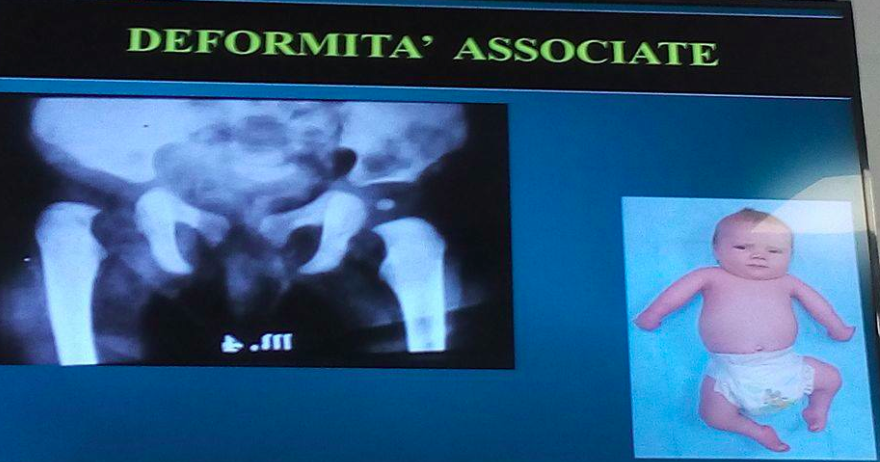
\includegraphics[width=0.4\textwidth]{016/image3.png}
\end{figure}

\subsubsection{Piede torto equino-cavo-varo-supinato}

È la forma clinica più frequente (65\% dei casi). Vengono prese in esame le possibili alterazioni sulle varie articolazioni coinvolte:

{[}Sono prese in esame \emph{tutte} le possibili alterazioni però quelle presenti in questa forma clinica sono appunto equinismo, varismo e supinazione{]}

\begin{itemize}
\item[1.]
  Alterazioni \textbf{\emph{sulla tibio-tarsica}} dove si osserva:
\begin{itemize}
\item
  \textbf{\emph{Equinismo}}: \emph{è una condizione di eccessiva flessione plantare rispetto alla gamba tale per cui l'appoggio del piede avviene solo con la porzione anteriore (\textbf{appoggio digitigrado}) come se il paziente camminasse sempre sulle punte. Il \emph{talismo} invece è una condizione di eccessiva flessione dorsale del piede tale da determinare l'appoggio solo sul retropiede come se il soggetto camminasse sempre sui talloni. }
\item
  \emph{Angolo retto tra piede e gamba}
\item
  \emph{Talismo}\textbf{:} \emph{è una condizione contrario all'equinismo infatti consiste in un'eccessiva flessione dorsale del piede tale da determinare l'appoggio solo sul retropiede come se il soggetto camminasse sempre sui talloni.}
\end{itemize}

\begin{figure}[!ht]
\centering
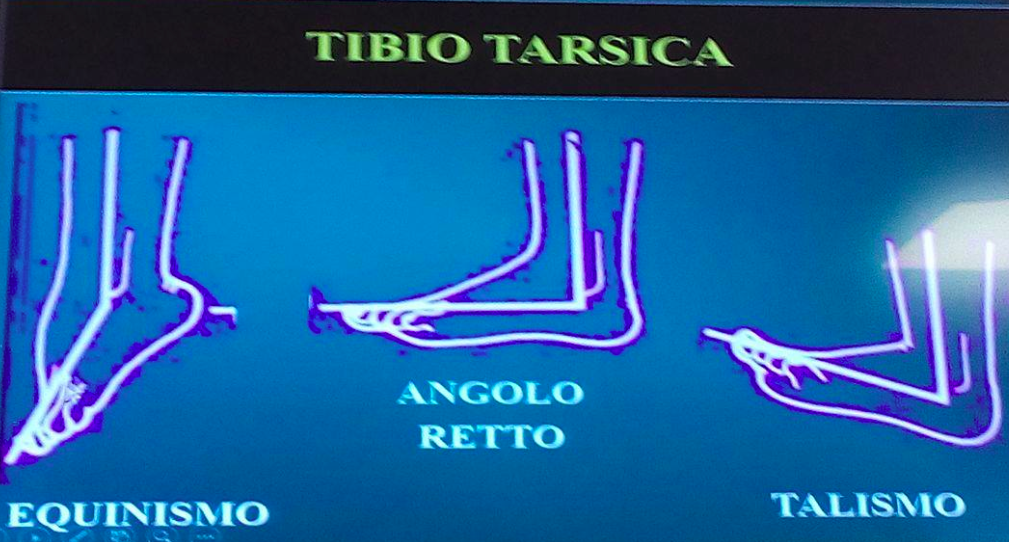
\includegraphics[width=0.4\textwidth]{016/image4.png}
\end{figure}

Immagine: \emph{Equinismo e talismo sono condizioni tra loro opposte, ma che riconoscono come causa un'alterazione anatomica a livello dell'\emph{articolazione tibio-tarsica}.}

\begin{figure}[!ht]
\centering
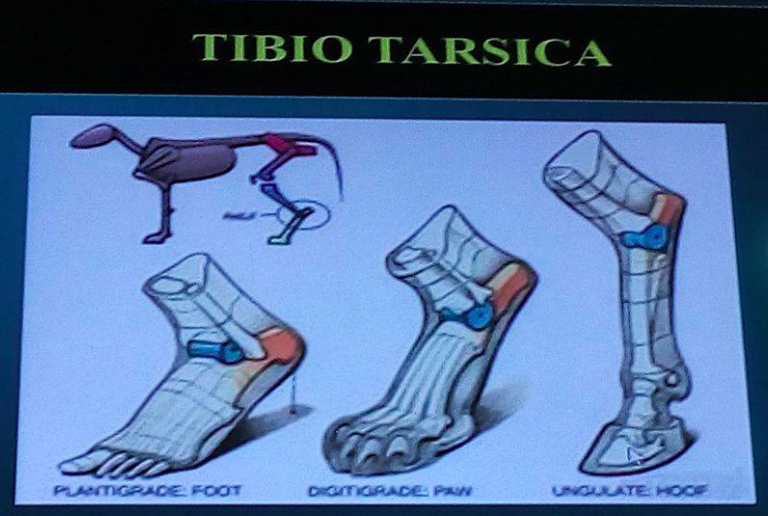
\includegraphics[width=0.4\textwidth]{016/image5.png}
\end{figure}

Perché si chiama equinismo?

Piccola digressione di anatomia comparata.

Nel piede di equino c'è un appoggio sulle dita (appoggio
\textbf{digitigrado}), lo zoccolo è l'unghia.

\begin{figure}[!ht]
\centering
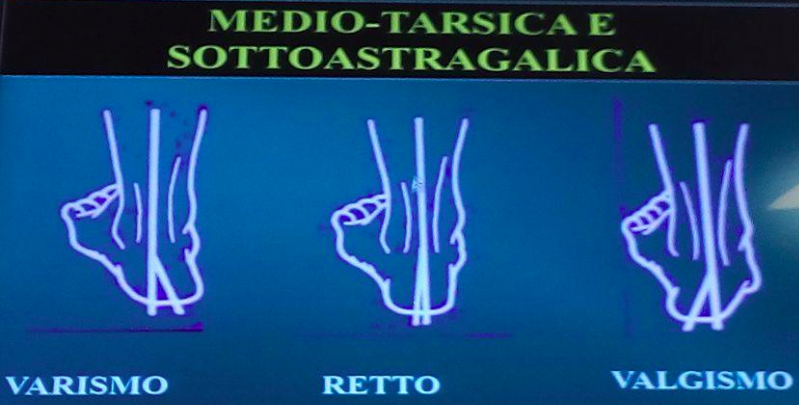
\includegraphics[width=0.4\textwidth]{016/image6.png}
\end{figure}

\item[2.]
  Alterazioni \textbf{sulla medio-tarsica} e \textbf{sottoastragalica}. È bene considerare insieme queste due articolazioni perché funzionalmente correlate. Si osserva\textbf{:}

\begin{itemize}
\item
  \textbf{\emph{Varismo}:} \emph{è una condizione dovuta ad una deviazione in senso mediale dell'asse longitudinale del piede. Il tallone va all'interno} perciò l'avampiede varo è ``sterzato'' all'interno ovvero addotto
\item
  \emph{Retropiede retto o leggermente valgo} (normalmente il valgo fisiologico è 5-7 gradi). \emph{Dall'immagine si può apprezzare come il varismo del retropiede si estrinsechi sia sulla medio tarsica e sotto astragalica quindi articolazione tra astragalo-calcagno, ma anche tra astragalo-calcagno-scafoide e cuboide.}
\item
  \emph{Valgismo (netto)}: come nel varismo c'è una deviazione dell'asse longitudinale del piede però in senso laterale; rispetto alla condizione di retropiede retto, la deviazione supera i 5-7 gradi. L'avampiede valgo è abdotto perché si allontana dalla linea mediana del corpo. \emph{Come nel piede piatto porta il piede ad un appoggio sulla parte interna}

\begin{figure}[!ht]
\centering
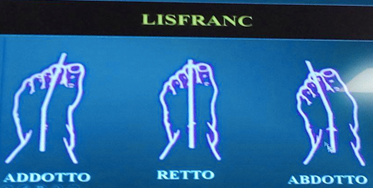
\includegraphics[width=0.4\textwidth]{016/image7.png}
\end{figure}

\end{itemize}
\end{itemize}

N.B. Varismo e valgismo sono legate ad alterazioni dell'articolazione medio-tarsica però opposte mentre per quanto riguarda l'articolazione sotto-astragalica:

\begin{itemize}
\item
  \emph{La \emph{supinazione} indica una rotazione del piede attorno al suo asse longitudinale così che la pianta del piede sia rivolta medialmente e l'appoggio al suolo avvenga solo sul bordo esterno. }
\item
  \emph{La \emph{pronazione} invece è l'opposto cioè una rotazione del piede tale da determinare che la faccia del piede sia rivolta lateralmente e l'appoggio del piede avvenga solo sul bordo interno. }
\end{itemize}

Quindi, nell'equino varo supinato abbiamo una \textbf{\emph{rotazione interna del tallone}}.

\begin{figure}[!ht]
\centering
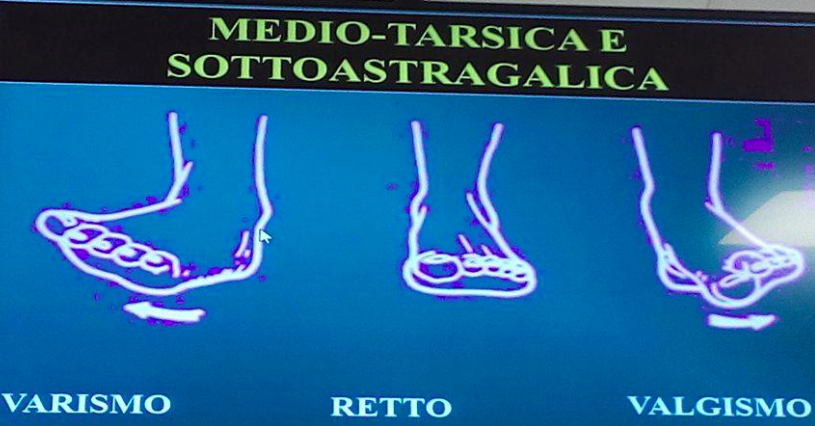
\includegraphics[width=0.4\textwidth]{016/image8.png}
\end{figure}

\begin{figure}[!ht]
\centering
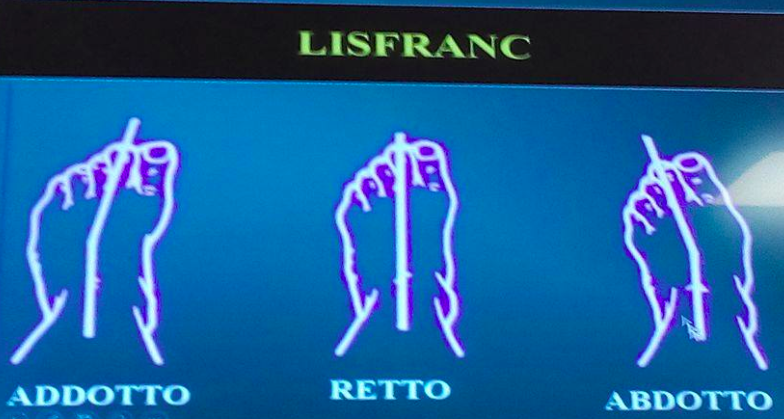
\includegraphics[width=0.4\textwidth]{016/image9.png}
\end{figure}

Qui si capisce bene come sono alterati i rapporti tra retropiede e avampiede.

\emph{L'atteggiamento del piede equino varo supinata sarà
contraddistinto da:}

\begin{itemize}
\item
  \emph{Equinismo}
\item
  \emph{Varismo}
\item
  \emph{Supinazione}
\item
  \emph{Callismo e adduzione dell'avampiede}
\item
  \emph{Retrazioni muscolo scheletriche prevalentemente nella parte interna del piede quindi tibiale posteriore, tibiale anteriore, flessore lungo delle dita, flessore lungo dell'alluce}
\item
  Un'alterazione dei rapporti tra le singole ossa che si estrinsecano con:

\begin{itemize}
\item
  Un perone più lungo
\item
  Un astragalo più orizzontale e più ruotato all'esterno
\item
  Un calcagno che va sotto l'astragalo
\item
  Uno scafoide che ``va a sbattere'' quasi sul malleolo interno.
\end{itemize}

Tali alterazioni dei rapporti ossei sono dovuti al fatto che nell'equino varo supinazione c'è una \textbf{retrazione} di tutto ciò che è \textbf{posteriore} (tendine di Achille, capsule articolari dell'articolazione tibiotarsica e della sottoastragalica, retrazione del tendine nel tibiale posteriore - nel flessore dell'alluce lungo e nel tibiale anteriore) e \textbf{mediale} con un'alterazione dei rapporti tra le ossa del piede.

Con l'accrescimento se questi rapporti tra le singole ossa vengono mantenuti alterati, le ossa si sviluppano in maniera altrettanto alterata.

Se non correggo l'equino, l'astragalo davanti cresce di più perché non si trova dentro la pinza tibio peroneale: il risultato è che il piede non torna su perché l'astragalo è molto più largo e quindi non entra più
nella pinza.
\end{itemize}

\begin{figure}[!ht]
\centering
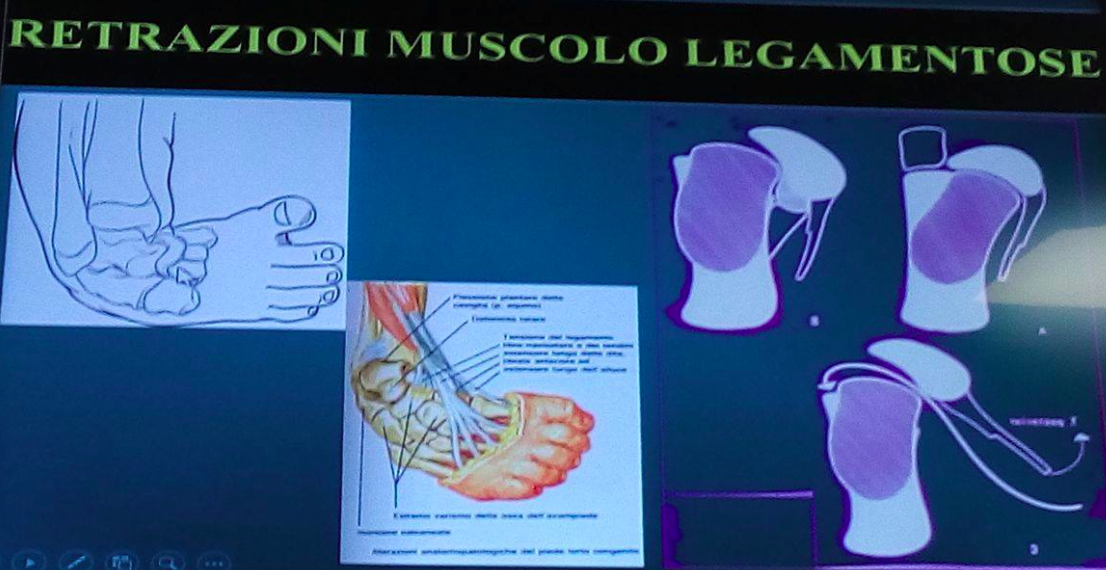
\includegraphics[width=0.4\textwidth]{016/image10.png}
\end{figure}

\paragraph{Diagnosi}

\begin{itemize}
\item[1.]
  Anamnesi
\item[2.]
  Esame clinico generale
\item[3.]
  Esame clinico del piede
\item[4.]
  Esame Rx del piede
\end{itemize}

Mostra un video (riportate alcune immagini significative) di un bambino tipicamente affetto da piede torto: sembra una forma sporadica perché non sembra essere un malformato.

Il suo atteggiamento è francamente eccessivo anche all'ispezione.

\begin{figure}[!ht]
\centering
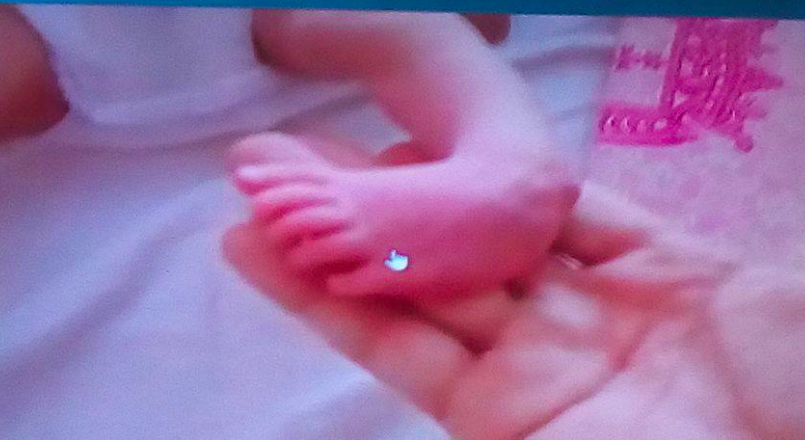
\includegraphics[width=0.4\textwidth]{016/image11.png}
\end{figure}

\begin{figure}[!ht]
\centering
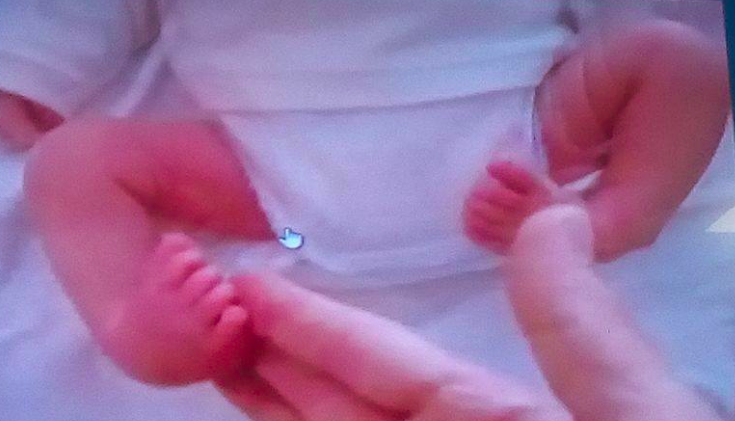
\includegraphics[width=0.4\textwidth]{016/image12.png}
\end{figure}

\paragraph{Esame clinico del piede}

\emph{La diagnosi del piede torto è facile: basta osservare il piede.
Dopo segue un esame clinico generale per esempio per vedere se c'è artrogriposi: non bisogna mai fermarsi solo al piede!} La prima cosa da vedere nel neonato è la \textbf{riducibilità della deformità} perché questo permette di chiarire la prognosi e l'eziologia. \emph{È infatti fondamentale capire la riducibilità perché dalla rigidità riusciamo a capire se è genetica o meccanica. Inoltre la rigidità risponde anche ad un criterio di tempo:} in funzione del tempo (accrescimento, età), ma
anche in funzione dell'eziologia, in tutte le forme abbiamo:

\begin{itemize}
\item
  \textbf{Fase della riducibilità}
\item
  \textbf{Fase della riducibilità relativa}
\item
  \textbf{Fase dell'irriducibilità}
\item
  \textbf{Piede torto inveterato}
\end{itemize}

Anche un piede torto sporadico che è riducibile all'inizio, se non trattato attraversa queste 4 fasi.

\emph{Più un bambino cresce non trattato, più si passa a una fase di riducibilità relativa fino ad arrivare a fasi di piede torto inveterato quando il paziente convive con la patologia da dieci anni e in questi casi vediamo enormi calli sulla parte esterna del piede.}

\emph{Spesso con la visione del piede si riesce a capire la gravità della situazione: se nel piede torto son presenti dei solchi, dei dermatoglifi geneticamente determinati e presenti in posizioni in cui non dovrebbero esserci, sono sintomatici di situazioni particolarmente
gravi e difficilmente risolvibili.}

Esempio di piedi torti non trattati: vediamo un appoggio non compatibile con una vita normale sia perché non è possibile indossare normali calzature sia per il dolore che ne consegue.

\begin{figure}[!ht]
\centering
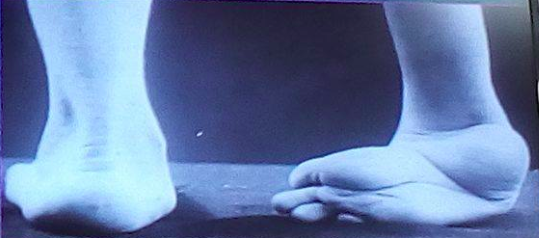
\includegraphics[width=0.4\textwidth]{016/image13.png}
\end{figure}

\paragraph{Esame radiografico}

L'esame radiografico conta poco nel piede torto perché non è possibile farlo prima dei 4-6-8 mesi di vita.

\emph{All'esame radiografico, nel piede piatto c'è l'astragalo in giù mentre nel piede cavo era più verticale. Nel piede torto l'astragalo è ai massimi livelli tanto è vero che nella proiezione dorso plantare le due ossa (astragalo e calcagno) si sovrappongono anziché avere un asse generalmente avrete proprio una sovrapposizione astragalo calcagno. }

\emph{Poi l'adduzione dell'avampiede (che va verso l'interno) porta ad un aumento di questo angolo però questa è la situazione radiologica dei piedi dell'immagine di sopra (quelli non trattati per anni) in cui addirittura i soggetti poggiano sull'astragalo sulla parte esterna.}

\begin{figure}[!ht]
\centering
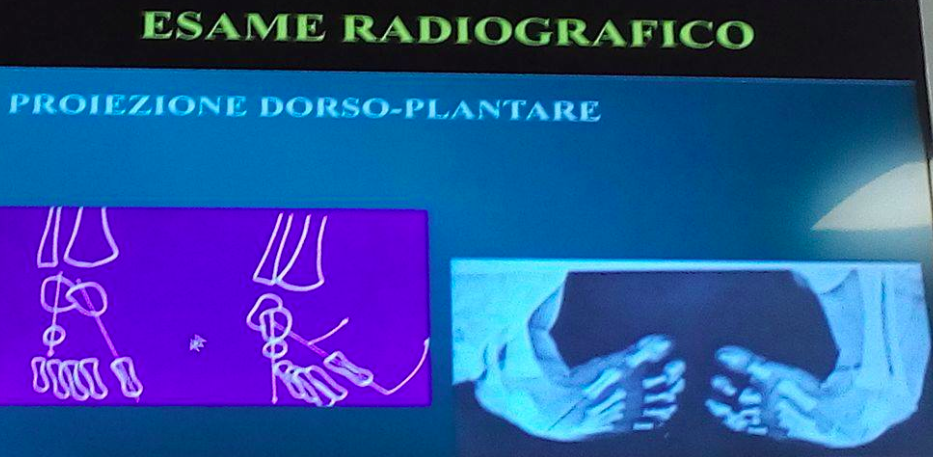
\includegraphics[width=0.4\textwidth]{016/image14.png}
\end{figure}

\paragraph{Trattamento}

Il trattamento può essere:

\begin{itemize}
\item
  \textbf{Ortopedico}
\item
  \textbf{Chirurgico}
\item
  \textbf{Combinato}: nella maggior parte dei casi
\end{itemize}

Prima vengono trattati, più aumentano le possibilità di guarigione per questi pazienti. L'obiettivo sarà correggere la deformità e cercare di mantenere la correzione. Prendiamo in esame le possibilità di
trattamento in relazione alla fase della deformità.

\begin{itemize}
\item[1.]
  Trattamento nella \emph{\textbf{FASE DELLA RIDUCIBILITA'}:}
	\begin{itemize}
\item
  Trattamento \textbf{ortopedico} mediante \textbf{manipolazioni} ovvero si cerca di contrastare quell'atteggiamento del piede in equino varismo supinazione. \emph{Le ossa di un bambino appena nato sono cartilaginee quindi il tendine d'Achille, il tibiale, hanno una resistenza meccanica nettamente superiore rispetto all'adulto per cui il rischio, forzando con queste manipolazioni, è quello di creare degli schiacciamenti e aggravare il quadro}. Queste manipolazioni devono essere:
		\begin{itemize}
\item
 \textbf{Precoci}: prima si inizia il trattamento meglio è
\item
  \textbf{Dolci e progressive}: nel neonato trazioni eccessive provocano degli schiacciamenti della cartilagine quindi successivamente lo sviluppo di ossa deformi
\item
  \textbf{L'equinismo è da correggere per ultimo e spesso per via chirurgica}: l'equinismo è l'espressione massima della deformità. Se provo a portare il piede su e a vincere l'equinismo in questa fase, il tendine di Achille, che è molto più resistente dell'astragalo cartilagineo, non si allunga. \emph{Dunque portando il piede ad angolo retto, questo avviene a spese di uno schiacciamento dell'astragalo che non sarà più tondo bensì piatto e di conseguenza la caviglia non si muoverà}
\item
  \textbf{Tali da considerare le retrazioni tendinee e legamentose.}
		\end{itemize}

\emph{Delle tre componenti (equinismo, varismo e supinazione) si manipolano solamente le ultime due ovvero varismo e supinazione. La componente equina non va manipolata.} Il pollice deve essere posizionato sulla testa dell'astragalo e \emph{si porta il piede (guarda immagine) fin quando non c'è resistenza e lo si immobilizza. Non bisogna andar oltre alla resistenza del tendine d'Achille. Se si applica troppa forza nelle manipolazioni, si hanno degli schiacciamenti delle ossa che possono portare ad un risultato non ottimale. }

\emph{Il risultato perfetto non esiste mai nel piede torto; è sempre molto difficile trovare il punto 0 (la normale posizione del piede).}

\emph{L'esito può essere un eccesso di pronazione proprio perché si va in ipercorrezione oppure si ha una recidiva (è possibile finché si ha l'accrescimento) magari di non tutte e 3 le componenti}

\emph{L'equinismo lo si risolve dopo chirurgicamente perché è impossibile ottenere l'allungamento del tendine d'Achille con sole manipolazioni. Si tratta il piede quando si arriva ad una situazione anestesiologicamente sopportabile, intorno ai 8-10 mesi, e si fa l'allungamento del tendine d'Achille.}

\begin{figure}[!ht]
\centering
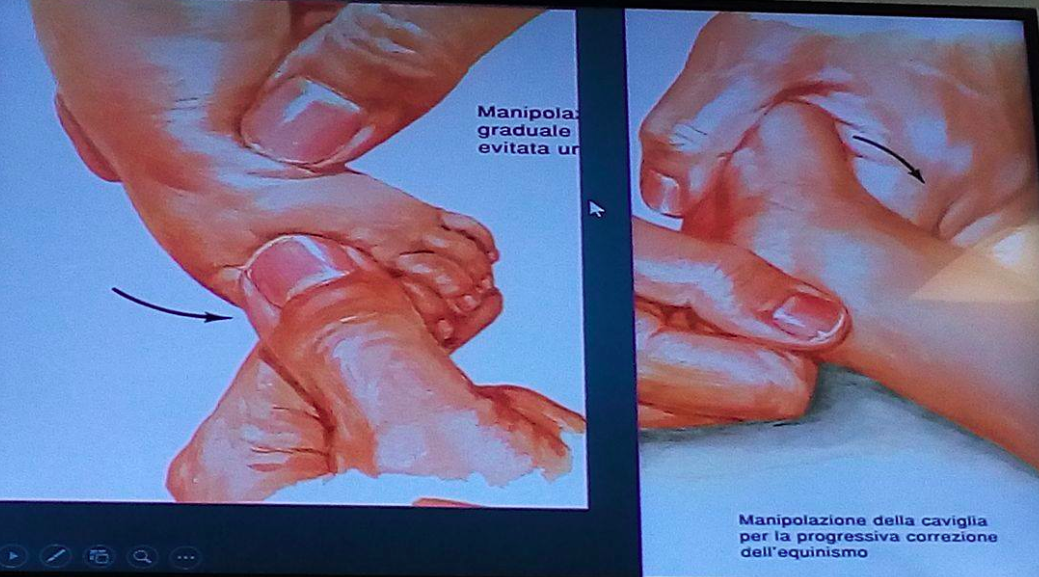
\includegraphics[width=0.4\textwidth]{016/image15.png}
\end{figure}

\begin{figure}[!ht]
\centering
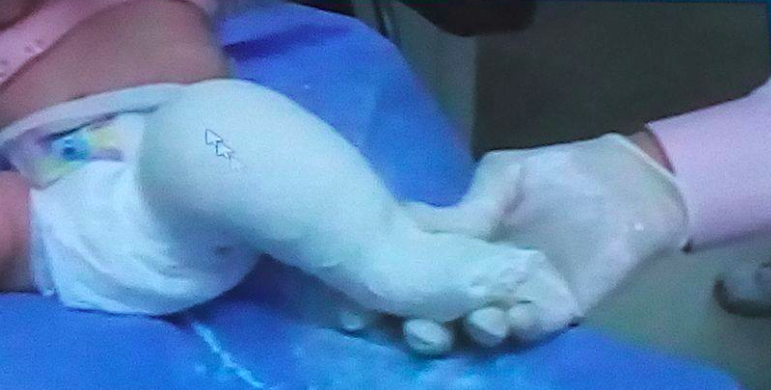
\includegraphics[width=0.4\textwidth]{016/image16.png}
\end{figure}

\begin{figure}[!ht]
\centering
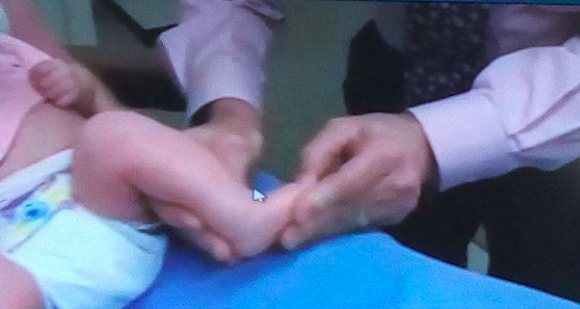
\includegraphics[width=0.4\textwidth]{016/image17.png}
\end{figure}

Eseguita la manipolazione vengono confezionati \textbf{apparecchi gessati}:

		\begin{itemize}
\item
  Da applicare dopo le manipolazioni
\item
  \textbf{In correzione} nel tentativo di mantenere la correzione che si è realizzata con la manipolazione. Così facendo si manterrà la correzione che tenderà a far cedere le parti molli (capsule e legamenti) dalla parte interna e posteriore
\item
  \textbf{Da sostituire ogni 15-20 giorni} per 2 motivi:

			\begin{itemize}
			\item
  			Man mano che si fanno le manipolazioni il gesso stabilizza una correzione sempre maggiore
			\item
  			Il neonato cresce molto rapidamente quindi se il gesso non viene sostituito il piede va in ischemia per compressione dei vasi oppure si ha compressione dei nervi (compressioni dell'arteria tibiale anteriore -> necrosi).

			N.B. Se si sfila il gesso, bisogna portare subito in ospedale il bambino (avvertire i genitori), perché va tolto subito.
			\end{itemize}
		\end{itemize}

\item
  Trattamento sempre \textbf{ortopedico} mediante \textbf{metodo Ponseti}. È un'altra opzione e non prevedere il trattamento chirurgico. Si tratta di manipolazioni che possono portare alla correzione anche senza intervento chirurgico ed anche nelle forme molto rigide. I gessi in questo caso di solito sono alti
  
\begin{figure}[!ht]
\centering
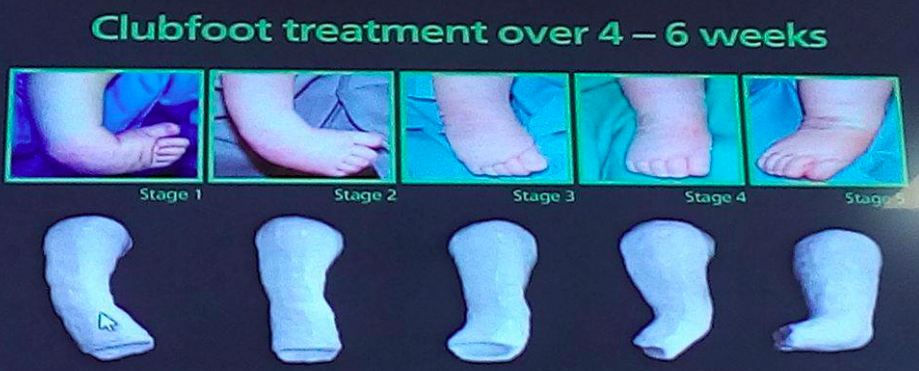
\includegraphics[width=0.4\textwidth]{016/image18.png}
\end{figure}

\item
  Trattamento \textbf{chirurgico} mediante due procedure\textbf{: Allungamento del tendine di Achille o Allungamento percutaneo}

	\begin{itemize}
\item
  \textbf{Allungamento del tendine di Achille:} Sulla componente di equinismo si agisce con l'allungamento del tendine di Achille. Si procede con un'incisione a Z: taglio longitudinale e due tagli orizzontali. A questo punto si esegue l'allungamento: il tendine viene sfibrato in due parti e si creano due monconi (emi tendini) che vengono suturati l'uno sull'altro. In genere a questo punto il piede viene su (lo piego ad angolo retto) e si realizzano in aggiunta anche delle capsulotomie posteriori. Bisogna stare molto attenti all'arteria tibiale posteriore che è l'arteria più importante di tutto il piede. Infine si separano con due forbicine e si aprono le due articolazioni (tibiotarsica e sottoastragalica posteriormente) così da migliorare l'equinismo.

\begin{figure}[!ht]
\centering
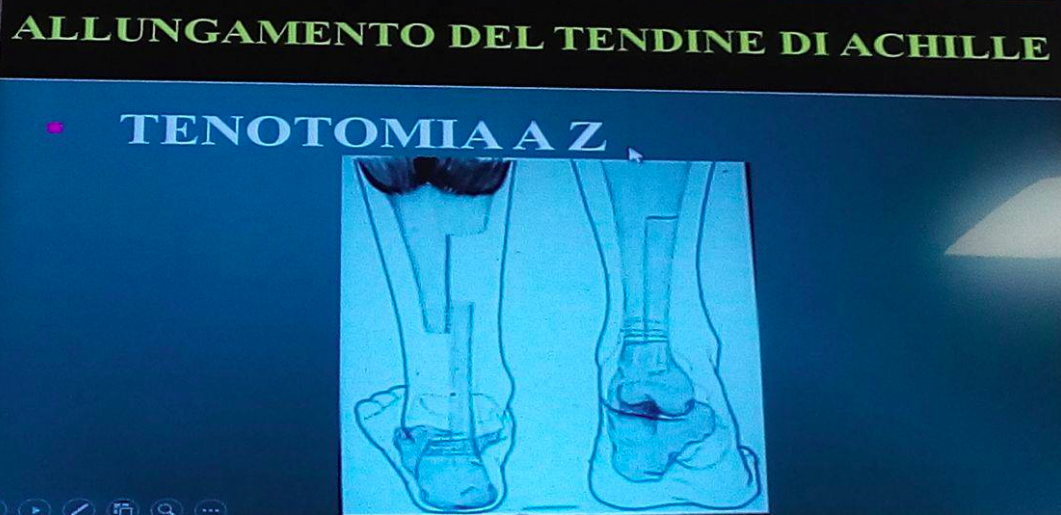
\includegraphics[width=0.4\textwidth]{016/image19.png}
\end{figure}

Osservare l'immagine sotto: la procedura si può considerare eseguita correttamente se si è raggiunto l'angolo retto. \emph{A quel punto si mette il gesso ad angolo retto; questi apparecchi vanno cambiati finché
il bambino non ricomincia a camminare}

\begin{figure}[!ht]
\centering
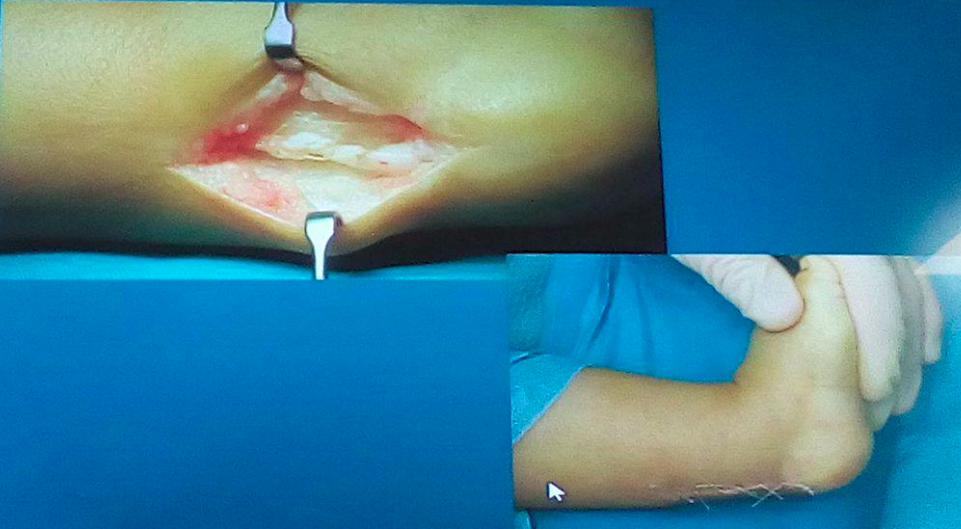
\includegraphics[width=0.4\textwidth]{016/image20.png}
\end{figure}

\begin{figure}[!ht]
\centering
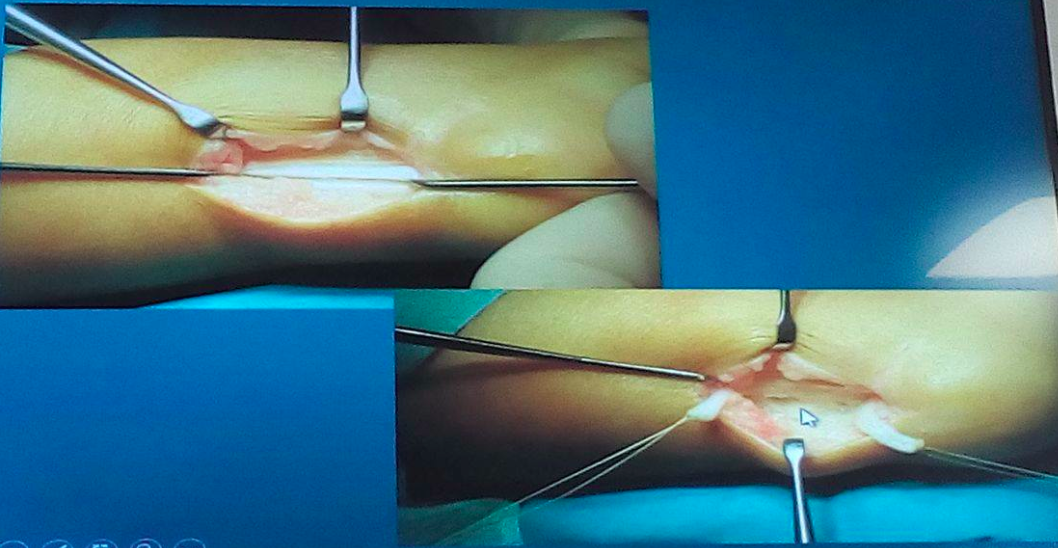
\includegraphics[width=0.4\textwidth]{016/image21.png}
\end{figure}

Vediamo che c'è una discreta riduzione di tutte le componenti.

Nell'immagine di sotto esempio di gesso post-operatorio.

\begin{figure}[!ht]
\centering
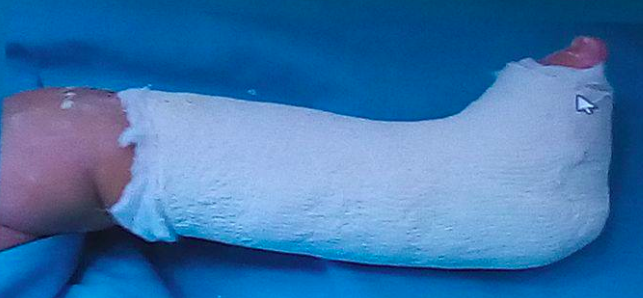
\includegraphics[width=0.4\textwidth]{016/image22.png}
\end{figure}

\item
  \textbf{Allungamento percutaneo}: È possibile anche un allungamento percutaneo: tagliando di netto con il bisturi. La possibilità di eseguire la procedura è legata all'età del paziente.
	\end{itemize}
\end{itemize}

\begin{figure}[!ht]
\centering
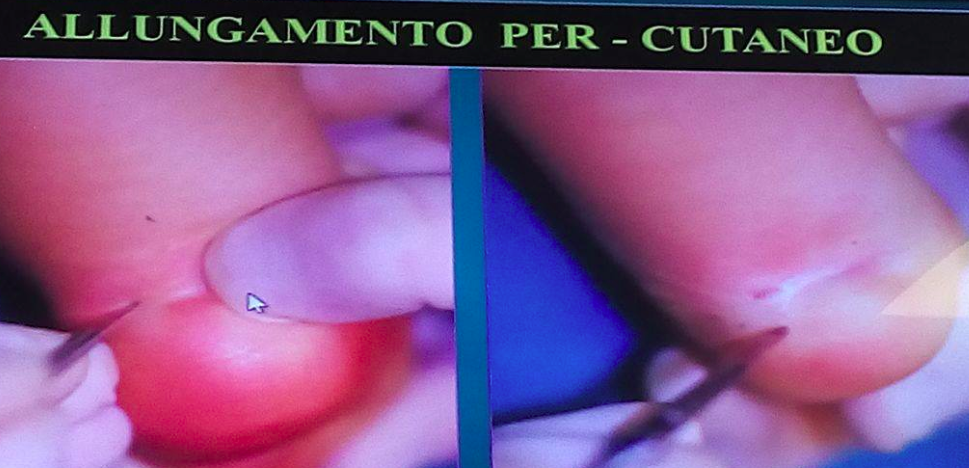
\includegraphics[width=0.4\textwidth]{016/image23.png}
\end{figure}

Siccome c'è una componente probabilmente genetica, \textbf{il piede torto è una deformità che tende a recidivare durante tutto il periodo dell'accrescimento} \emph{e quindi bisogna continuare il trattamento.
Innanzitutto si utilizzazione delle \emph{docce di posizione }}che vengono portare a seconda dell'età:

\begin{figure}[!ht]
\centering
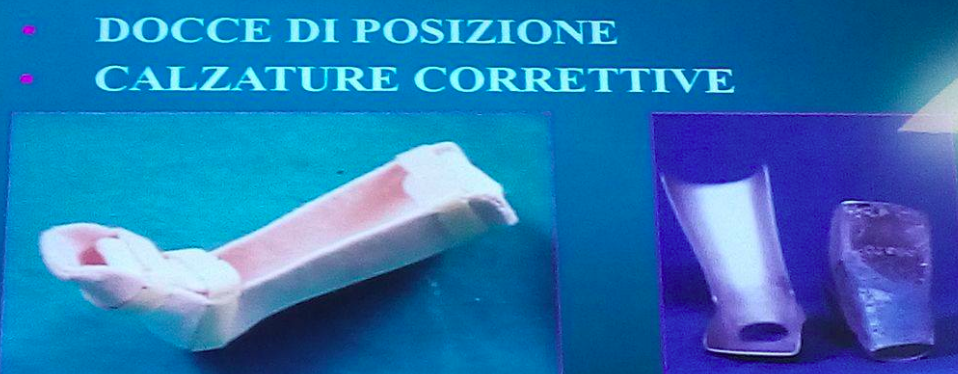
\includegraphics[width=0.4\textwidth]{016/image24.png}
\end{figure}

\begin{itemize}
\item
  Tutto il giorno se il bambino non cammina
\item
  Solo di notte se cammina
\item
  Durante il giorno se si usano calzature correttive
\end{itemize}

Infine possono essere utilizzate anche delle \emph{calzature correttive:}

\begin{itemize}
\item
  \textbf{Scarpa Bebax}: inventata negli anni 90, è usata poco perché non ha la presa di gamba. Permette di variare il rapporto tra retropiede ed avampiede attraverso snodi che sbloccano con delle viti a brugola. Può andare bene in un metatarso varo.

\begin{figure}[!ht]
\centering
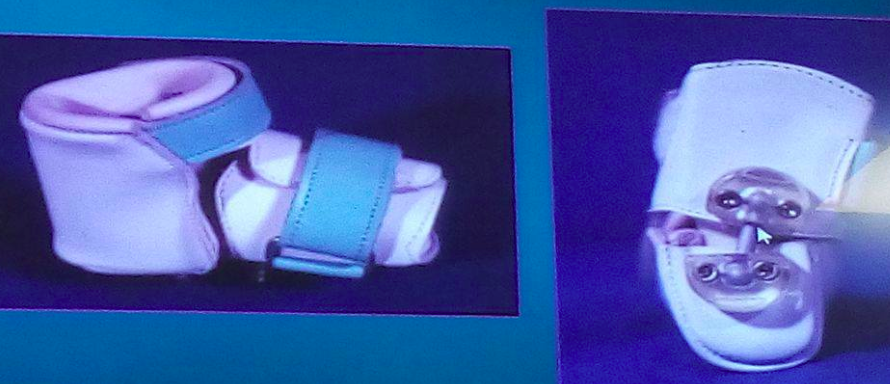
\includegraphics[width=0.4\textwidth]{016/image25.png}
\end{figure}

\item
  Nella \textbf{scarpa a biscotto} non c'è distinzione tra destra e sinistra. Questa scarpa funziona con il principio dei 3 punti: la spinta sulla convessità e la controspinta sui due estremi: una spinta a livello del cuboide, una spinta a livello della testa del primo metatarso e una spinta a livello del tallone in maniera tale da ``sterzare'' l'adduzione dell'avampiede. Si tratta di scarpe ortopediche.

\begin{figure}[!ht]
\centering
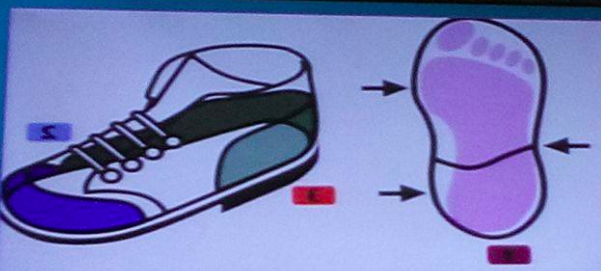
\includegraphics[width=0.4\textwidth]{016/image26.png}
\end{figure}

\end{itemize}

\item[2.]
  Trattamento nella \textbf{FASE DELLA RIDUCIBILITA' RELATIVA}. È un trattamento solo chirurgico: intervento \textbf{di Codivilla}

In questa fase il piede è più resistente \emph{e solo parzialmente riducibile} per cui il trattamento può essere solo chirurgico. Non si riuscirà a ridurlo con le manipolazioni.

\begin{figure}[!ht]
\centering
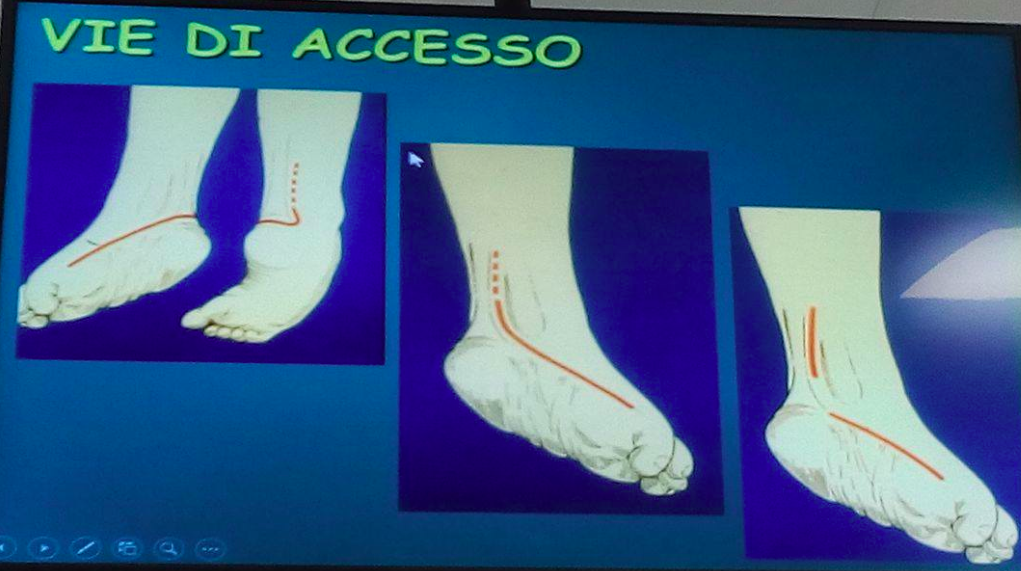
\includegraphics[width=0.4\textwidth]{016/image27.png}
\end{figure}

\begin{figure}[!ht]
\centering
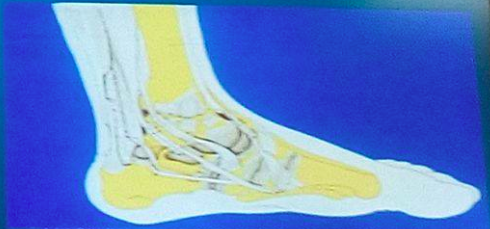
\includegraphics[width=0.4\textwidth]{016/image28.png}
\end{figure}

L'intervento prevede:

\begin{itemize}
\item
  \emph{Doppia incisione chirurgica: una nella parte posteriore e una nella parte interna del piede} (vedi immagine ``vie di accesso'')
\item
  Per prima cosa occorre \emph{isolare} con un elastico \emph{il fascio vascolo-nervoso} per evitare lesioni (nervo tibiale posteriore, arteria tibiale posteriore)

\begin{figure}[!ht]
\centering
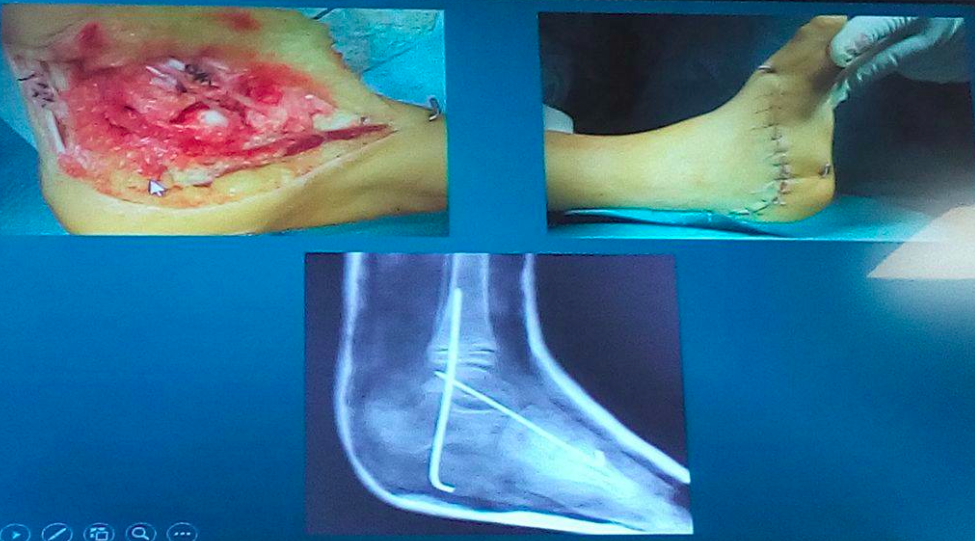
\includegraphics[width=0.4\textwidth]{016/image29.png}
\end{figure}

\begin{figure}[!ht]
\centering
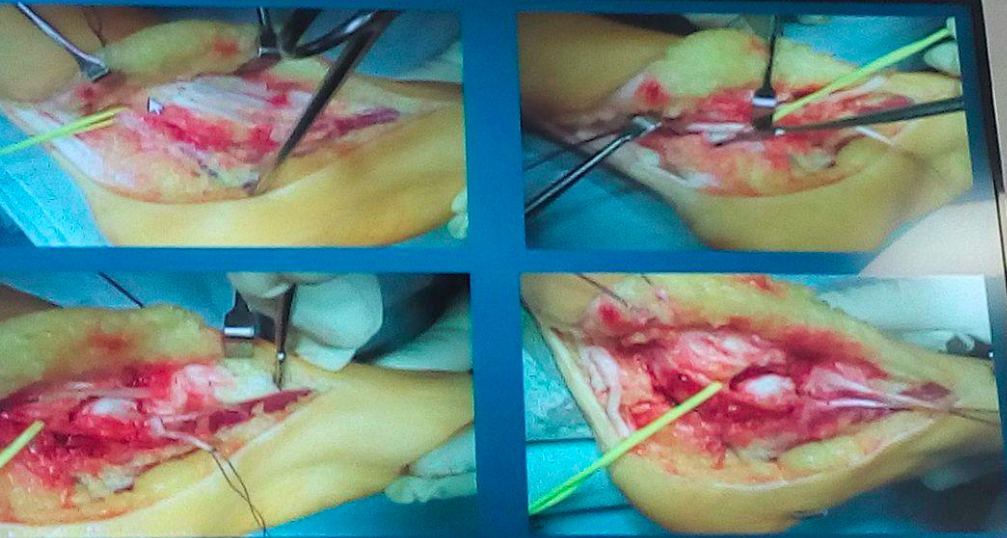
\includegraphics[width=0.4\textwidth]{016/image30.png}
\end{figure}

\begin{figure}[!ht]
\centering
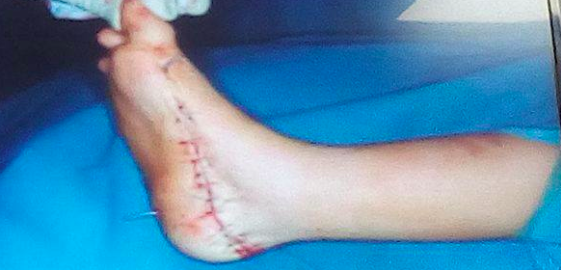
\includegraphics[width=0.4\textwidth]{016/image31.png}
\end{figure}

\item
  Vengono eseguiti
  \begin{itemize}
    \item
    \emph{Allungamenti plastici di tutti i tendini della parte mediale} del piede (tibiale anteriore, tibiale posteriore, flessore lungo dell'alluce, flessore delle dita),
  \item
    \emph{\emph{Tenotomia Achillea:}} allungamento del tendine d'Achille
  \item
    \emph{Capsulotomie mediali} di tutte le articolazioni della colonna interna (scafo-\emph{cuneiforme}, cuneo-metatarsale),
  \item
    \emph{Distacco dell'adduttore}.
\end{itemize}
\end{itemize}

Le varie incisioni sono molto ampie per permettere tutti gli allungamenti necessari.

Bisogna ridurre i rapporti tra le singole ossa.

I \textbf{fili di Kirschner} aiutano per circa un mese a tenere il giusto rapporto tra scafoide e astragalo.

Si tratta di tagli che lasciano grosse cicatrici anche non perfette.

Una volta che ridiamo i giusti rapporti, le ossa si ristrutturano tra di loro (visibile nella RX) perché soprattutto nella fase dell'accrescimento c'è una capacità di rimodellamento dell'osso.

\emph{Al termine viene confezionato un apparecchio gessato lungo fino alla radice della coscia che mantiene la correzione ottenuta. Il gesso viene portato fino al successivo controllo che avviene dopo 12/15 giorni e in cui avviene la sostituzione dell'apparecchio gessato. Intorno all'8-9 mese di età vengono dunque confezionate delle calzature ortopediche, definite ``a biscotto'' che manterranno la correzione. Il destino prognostico è strettamente correlato non solo alla precocità ed alla razionalità del trattamento, ma anche all' entità della
deformazione iniziale ed alla capacità riparativa del piede deforme. Non va dimenticato comunque che la deformità, essendo legata ad un arresto o ad un rallentamento dello sviluppo embrionale, tende a ripresentarsi ogni qual volta vi sia una spinta evolutiva all' accrescimento del piede, ragion per cui è necessaria una continua e stretta sorveglianza di questi pazienti per intervenire precocemente qualora si osservino i segni di un ripristino della deformità.}

Bambina di 9 anni con borsite della parte esterna -> intervento e controllo a distanza.

\begin{figure}[!ht]
\centering
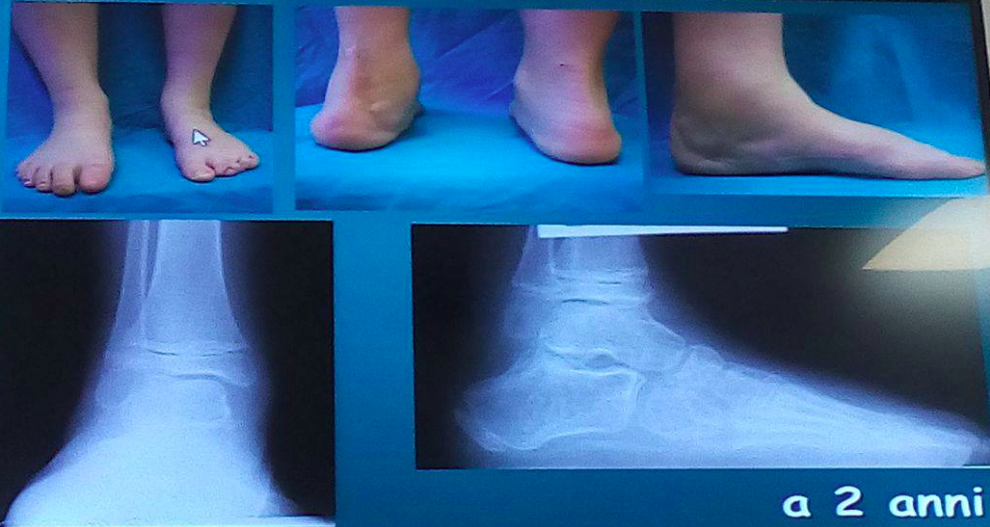
\includegraphics[width=0.4\textwidth]{016/image32.png}
\end{figure}

Dopo correzione ha una rotazione di circa 12 gradi, ma comunque si preferisce un piede così rispetto a come era prima della correzione.

Se correggiamo poco un piede, l'accrescimento successivo dà una recidiva (figura a sx).

Se lo correggiamo troppo viene un piede piatto (figura a dx).

\begin{figure}[!ht]
\centering
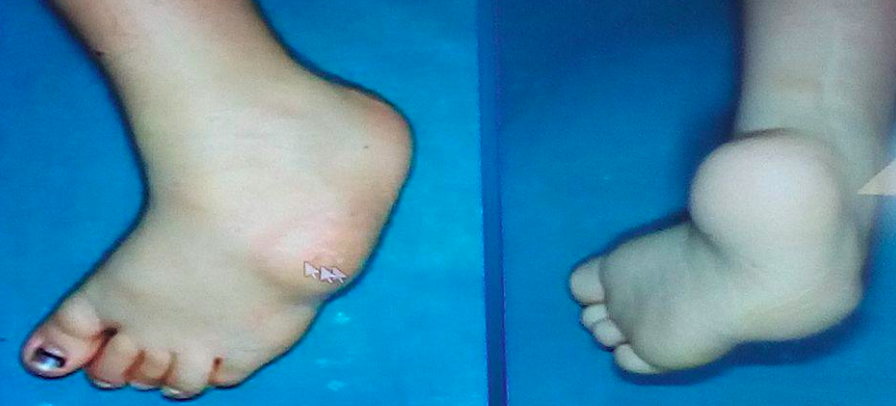
\includegraphics[width=0.4\textwidth]{016/image33.png}
\end{figure}

\begin{figure}[!ht]
\centering
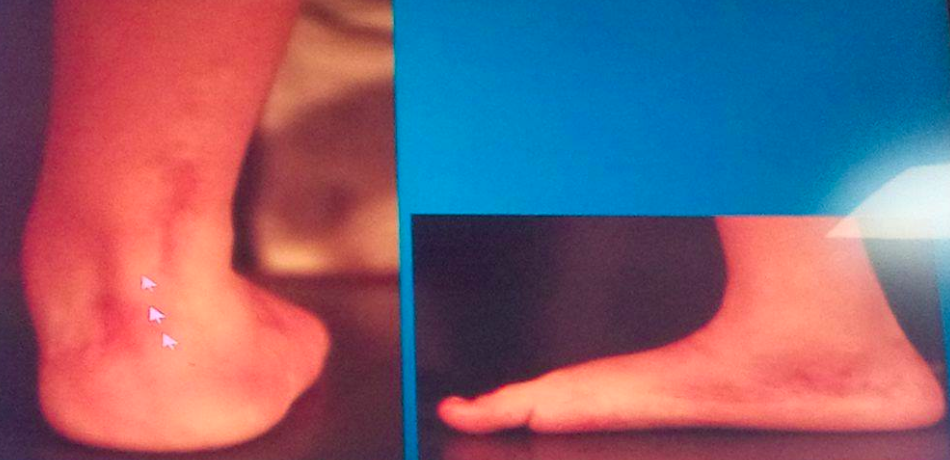
\includegraphics[width=0.4\textwidth]{016/image34.png}
\end{figure}

\item[3.]
  Trattamento nella \textbf{\emph{FASE DELL'IRRIDUBILITA'}}. Il trattamento è solo chirurgico e bisogna intervenire non solo sulle parti molli, ma anche sullo scheletro con \textbf{artrodesi} od \textbf{osteotomie}.

\begin{figure}[!ht]
\centering
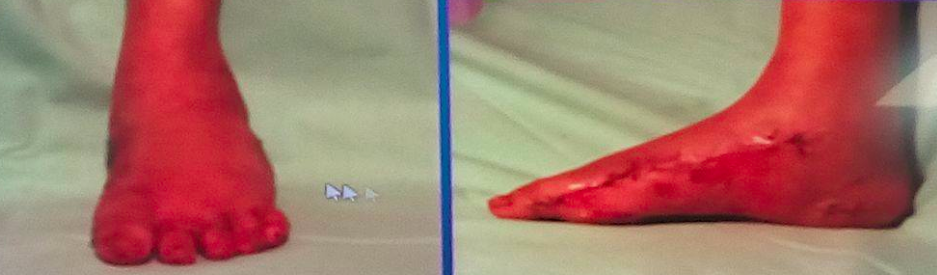
\includegraphics[width=0.4\textwidth]{016/image35.png}
\end{figure}

\begin{figure}[!ht]
\centering
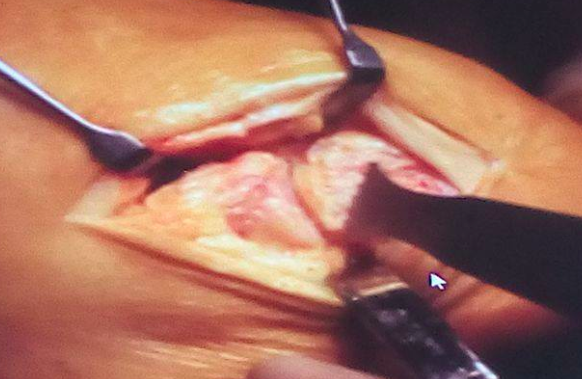
\includegraphics[width=0.4\textwidth]{016/image36.png}
\end{figure}

\begin{figure}[!ht]
\centering
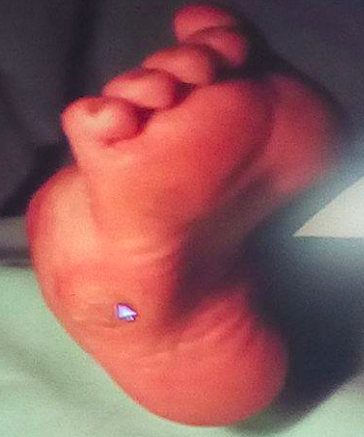
\includegraphics[width=0.4\textwidth]{016/image37.png}
\end{figure}

\item[4.]
  Trattamento del \textbf{\emph{PIEDE TORTO INVETERATO.}} Quando il piede è già inveterato, c'è già un'artrosi ed è rigido, non si riesce a far nulla. In questo caso l'unica possibilità è quella \textbf{chirurgica}. Si esegue una \textbf{duplice artrodesi}: si fanno dei cunei ossei e si cerca di riportare il piede nella giusta posizione per garantire un buono appoggio e permettere di indossare calzature normali.
  
\begin{figure}[!ht]
\centering
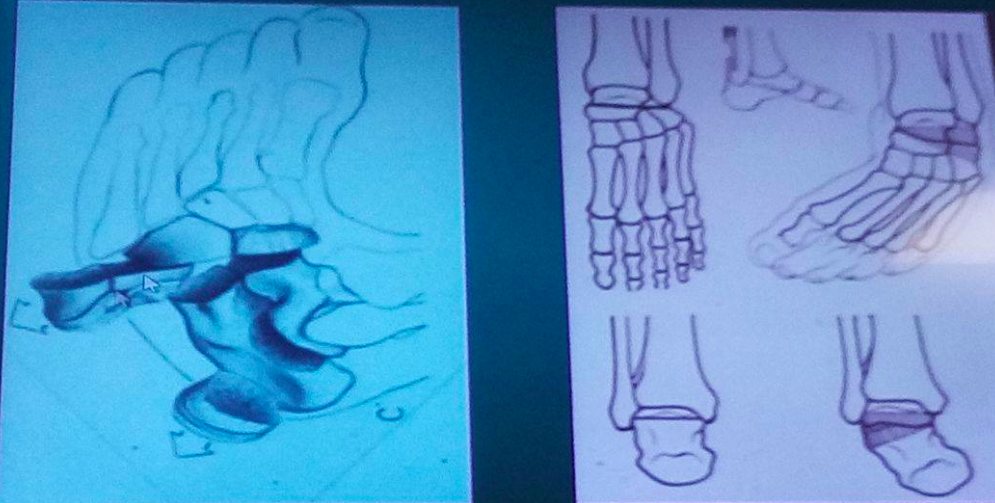
\includegraphics[width=0.4\textwidth]{016/image38.png}
\end{figure}

\begin{figure}[!ht]
\centering
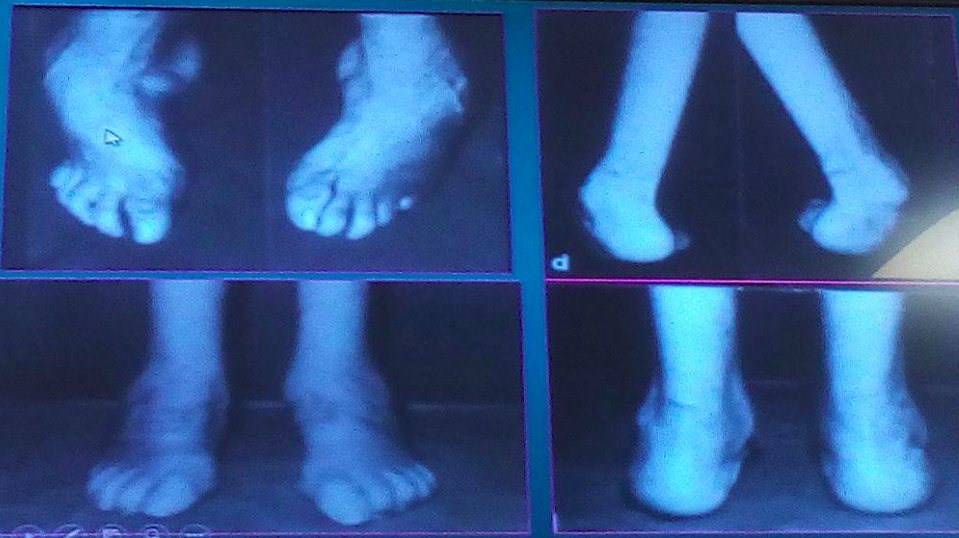
\includegraphics[width=0.4\textwidth]{016/image39.png}
\end{figure}

{[}Ragazzo di 27 anni{]}
\end{itemize}

\subsubsection{Piede talo valgo pronato}

\emph{Altra forma clinica caratterizzata da:}

\begin{itemize}
\item
  \emph{Talismo con flessione dorsale del piede}
\item
  \emph{Valgismo in quanto l'appoggio avviene solo sul calcagno che appare deviato lateralmente rispetto all'asse longitudinale della gamba}
\item
  \emph{Pronazione con l'avampiede ruotato sul suo asse longitudinale così che la pianta sia rivolta all'esterno }
\item
  \emph{Piattismo con l'appiattimento della volta plantare longitudinale.}
\end{itemize}

Nel neonato se ne vedono tanti e molto spesso si risolvono per conto loro: sono solitamente neonati flaccidi.

Anche qui si procede con \textbf{manipolazioni} ed \textbf{apparecchi gessati} in situazione opposta. \emph{Non c'è il problema del tendine d'Achille che è allungato e quindi possiamo mettere in posizione anche la terza componente (il talismo). Sono gessi fatti esattamente come se fosse un equino varo supinato.}

\emph{Si fa un trattamento chirurgico con appoggio sul calcagno: si impianta una stecca d'osso presa dalla tibia e messa in modo da limitare la dorsiflessione. In questo caso si ha una limitazione della mobilità della tibiotarsica,}

\begin{figure}[!ht]
\centering
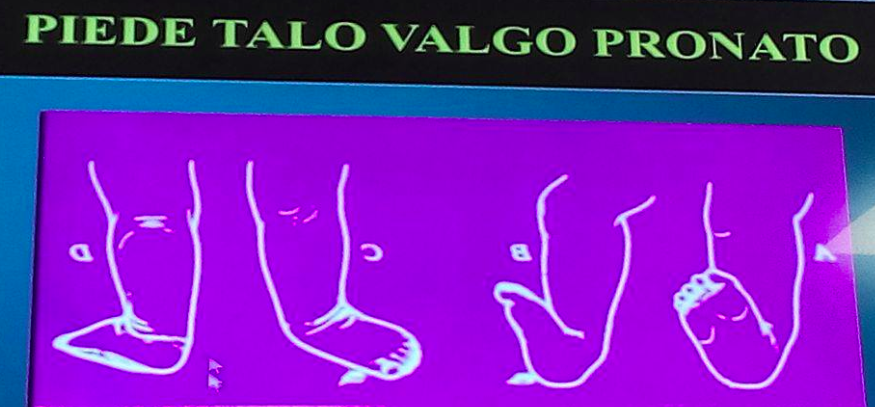
\includegraphics[width=0.4\textwidth]{016/image40.png}
\end{figure}

Ragazzo di 13 anni con piedi che vanno troppo in flessione dorsale, sono stati corretti attraverso una artrorisi (la flessione dorsale della caviglia è stata bloccata come spiegato sopra).

\begin{figure}[!ht]
\centering
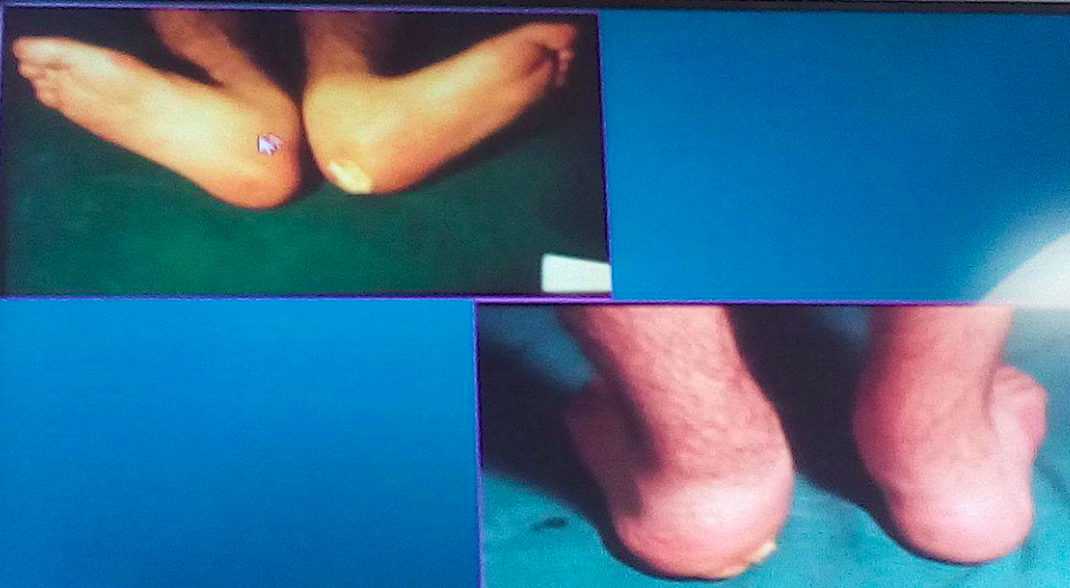
\includegraphics[width=0.4\textwidth]{016/image41.png}
\end{figure}

\begin{figure}[!ht]
\centering
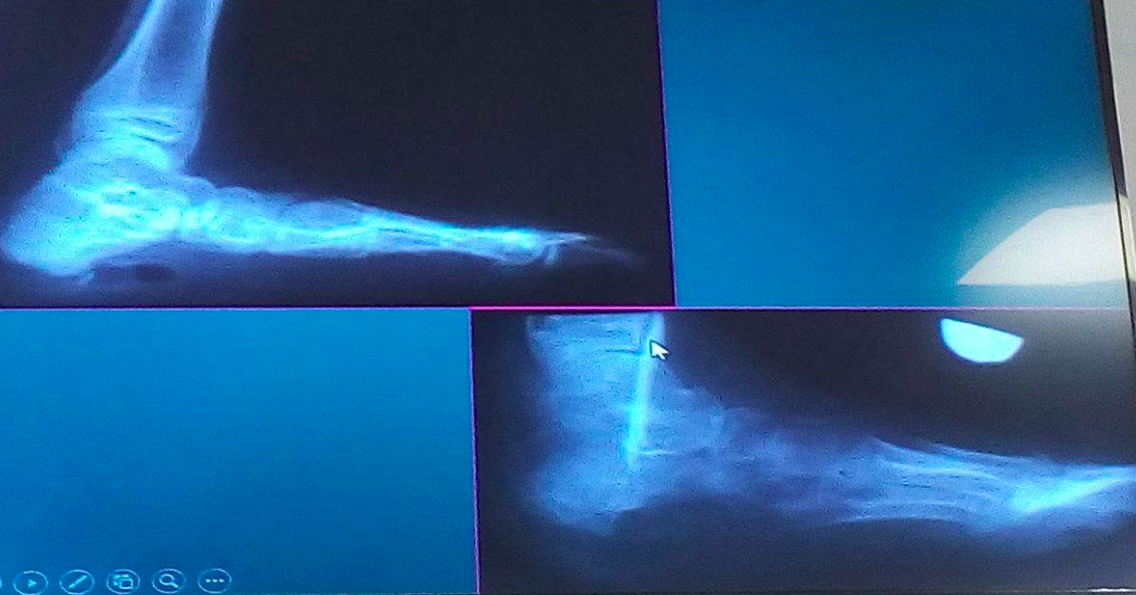
\includegraphics[width=0.4\textwidth]{016/image42.png}
\end{figure}

\subsubsection{Piede valgo-convesso (astragalo verticale)}

\emph{Rara deformità caratterizzata dall'inversione della volta plantare.}

\begin{figure}[!ht]
\centering
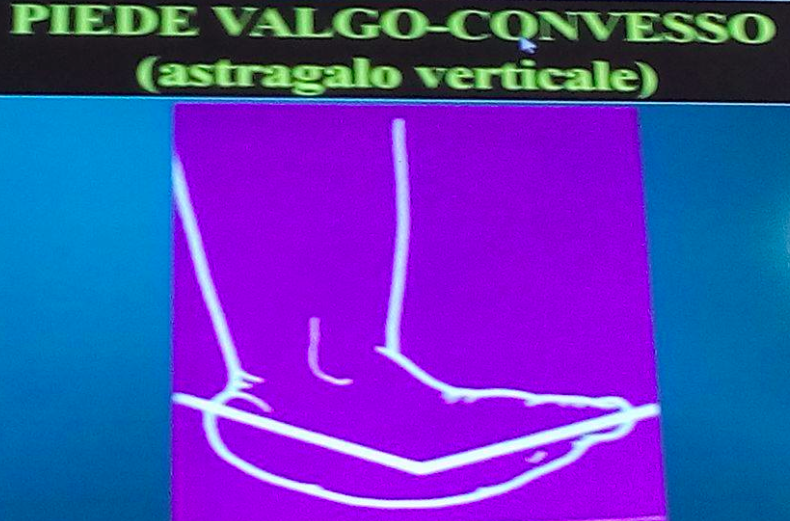
\includegraphics[width=0.4\textwidth]{016/image43.png}
\end{figure}

\begin{itemize}
\item
  C'è un \textbf{equinismo del retropiede} (il calcagno è in equinismo perché c'è una retrazione dell'Achille)
\item
  Ma \textbf{un avampiede che viene su}.
\item
  Caratteristica \emph{verticalizzazione dell'astragalo}
\item
  C'è un'inversione della volta plantare: il tallone non poggia per niente.
\end{itemize}

\begin{figure}[!ht]
\centering
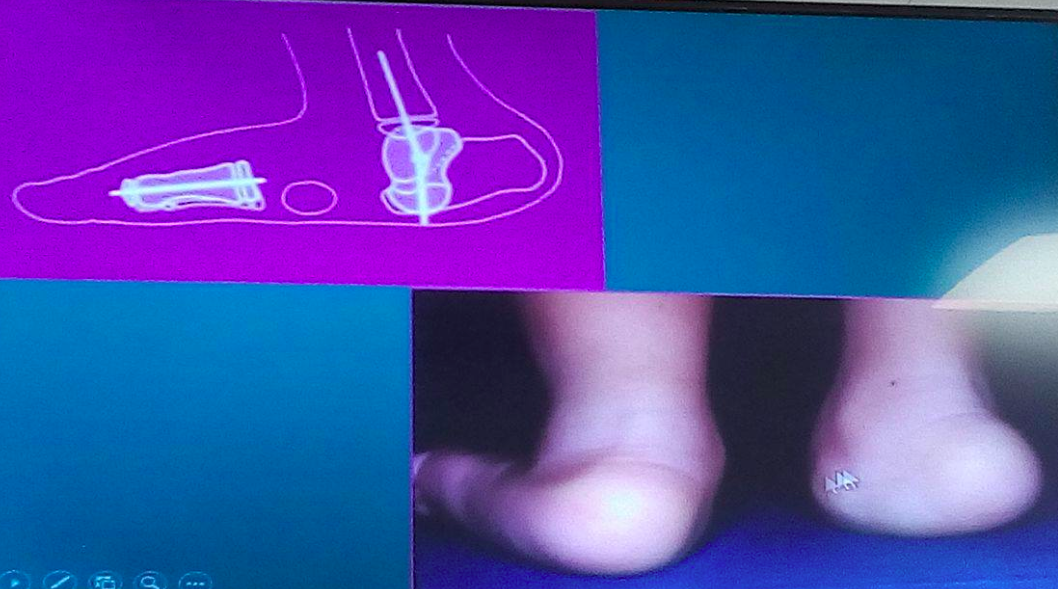
\includegraphics[width=0.4\textwidth]{016/image44.png}
\end{figure}

L'unico approccio è quello chirurgico. Si tratta di interventi enormi.
Ci sono varie vie di accesso e bisogna \emph{allungare i peronei}, il tendine di Achille e quindi riposizionare l'astragalo sullo scafoide e quest'ultimo è sempre il punto chiave dell'intervento. \emph{Dopo l'intervento l'astragalo non punta più in basso ed è ridotto sullo
scafoide, vengono spesso usati dei fili che vengono applicati con dei trapani, manipolati e poi rimossi in ambulatorio dopo l'intervento.}

\begin{figure}[!ht]
\centering
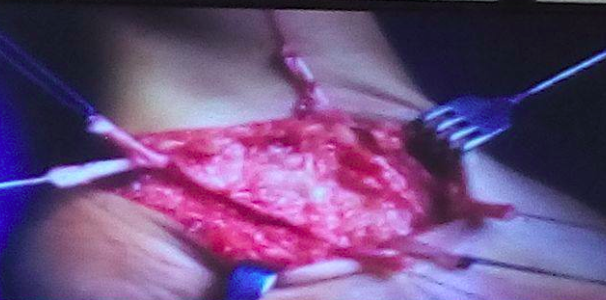
\includegraphics[width=0.3\textwidth]{016/image45.png}
\end{figure}

Nella lastra del postoperatorio si nota che l'astragalo, che prima era verticale, è stato rimesso in asse con la colonna interna del piede.

\begin{figure}[!ht]
\centering
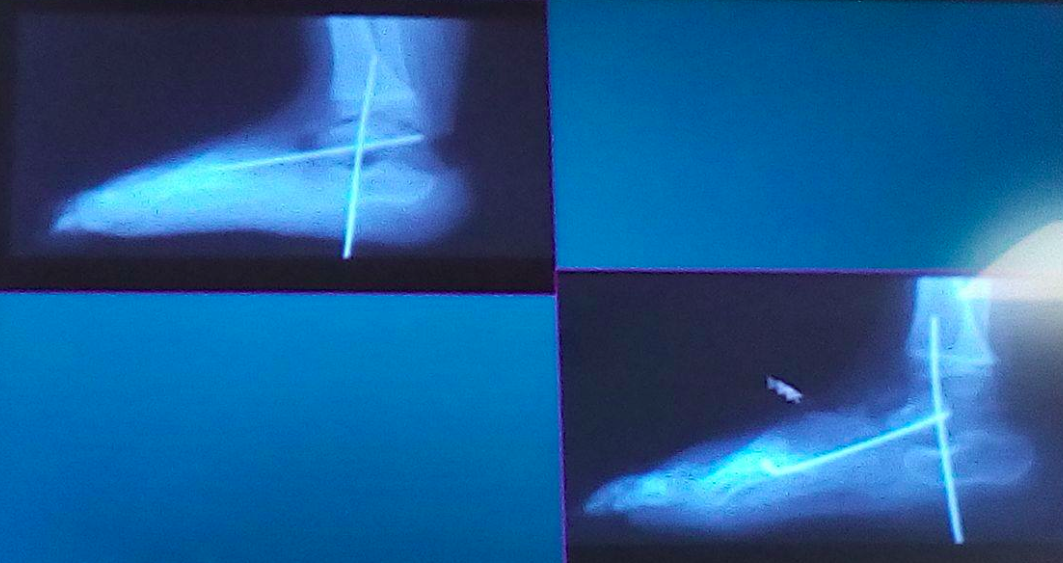
\includegraphics[width=0.3\textwidth]{016/image46.png}
\end{figure}

\begin{figure}[!ht]
\centering
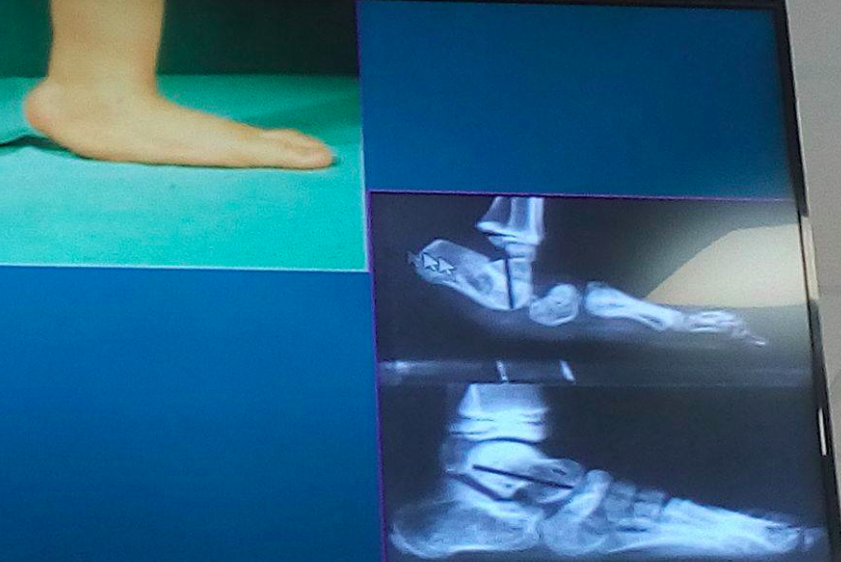
\includegraphics[width=0.3\textwidth]{016/image47.png}
\end{figure}

\subsubsection{Piede metatarso varo}

C'è una componente di \textbf{adduzione solo dell'avampiede}, tutto l'avampiede è sterzato.

Il retropiede è sostanzialmente normale. \emph{Si tratta di una delle maggiori cause di marcia a punta intra ruotate: i bambini camminano con la punta dei piedi. Questa andatura può dipendere da:}

\begin{itemize}
\item
  \emph{Un metatarso varo}
\item
  \emph{Un vizio di torsione dell'arto inferiore }
\item
  \emph{Un valgismo del collo femorale. Se c'è un valgismo del collo femorale e quindi un aumento dell'angolo tra diafisi e collo, c'è anche un aumento dell'angolo di inclinazione quindi la testa del femore guarda in avanti e il bambino automaticamente intra ruota tutto l'arto per centrare la testa del femore e quindi la marcia può essere un termometro per la displasia dell'anca. }
\end{itemize}

\emph{In Rx i metatarsali son tutti affastellati verso la mediale.
Chirurgicamente si fa poco: capsulotomie delle articolazioni mediali e soprattutto distacco del muscolo adduttore che è nella parte interna del piede. Si tratta di un intervento difficile perché vicino all'inserzione
passa l'arteria, quando sono più grandi bisogna accorciare la colonna esterna e allungare la colonna interna, si prende un pezzo d'osso dalla parte esterna e la si mette nella parte interna dove dobbiamo allungare, il tutto per esitare in un aggiustamento dei rapporti tra avampiede e
retropiede.}

\emph{Non è una situazione che rispetto al piede torto dia molto fastidio, qui tutto sommato quando si irrigidisce può dare qualche fastidio con le scarpe ma è molto meno frequente dover arrivare alla chirurgia.}

\begin{figure}[!ht]
\centering
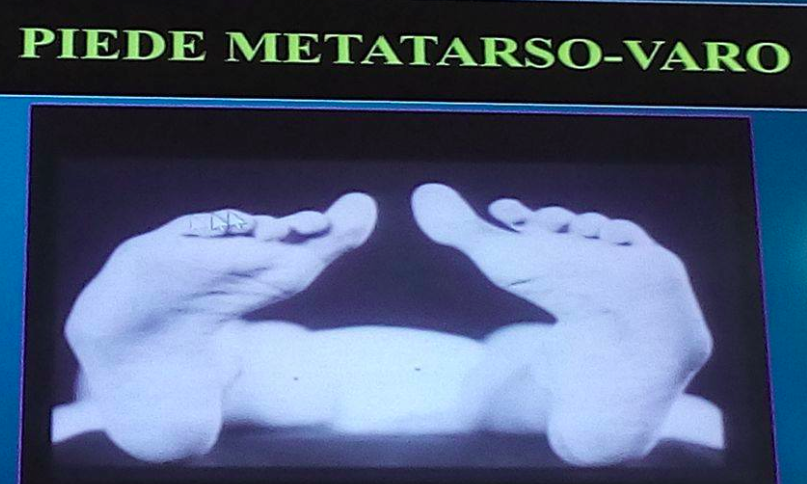
\includegraphics[width=0.3\textwidth]{016/image48.png}
\end{figure}

\begin{figure}[!ht]
\centering
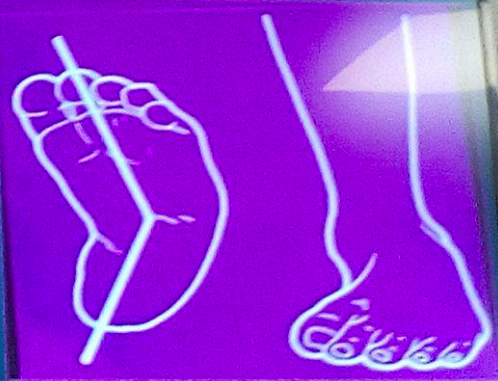
\includegraphics[width=0.3\textwidth]{016/image49.png}
\end{figure}

\begin{itemize}
\item
  Trattamento ortopedico:
\begin{itemize}
\item
  \textbf{Manipolazioni.} \emph{La componente di adduzione viene corretta con manipolazioni e apparecchi gessati: la manipolazione va fatta cercando di allungare la parte interna del piede, capsule e anche il muscolo adduttore.}
\item
  \textbf{Apparecchi gessati} \emph{per dominare l'adduzione.} Questi gessi poi vengono tagliati e man mano corretti.

\begin{figure}[!ht]
\centering
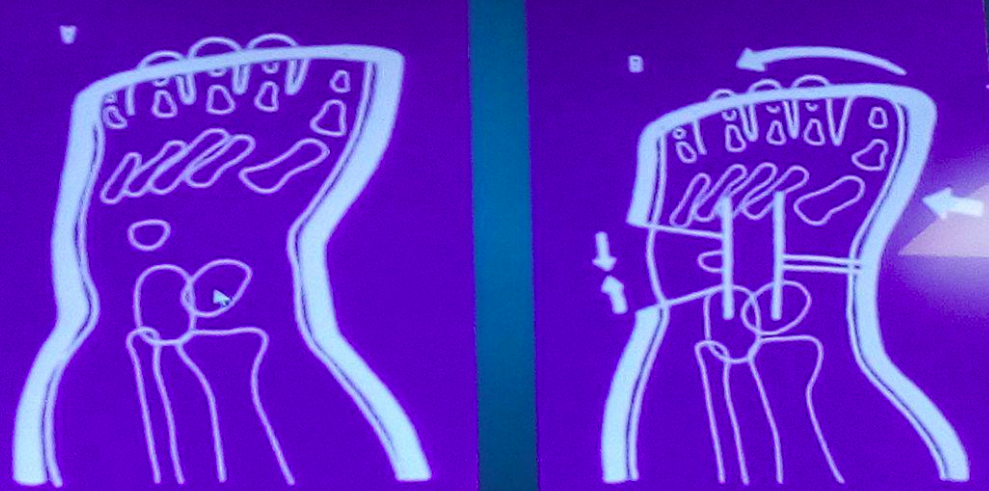
\includegraphics[width=0.3\textwidth]{016/image50.png}
\end{figure}

\item
  \textbf{Docce} per la notte, \textbf{scarpe a biscotto}.
\end{itemize}

\item
  Trattamento \textbf{chirurgico}. \emph{Chirurgicamente si fa poco: capsulotomie delle articolazioni mediali e soprattutto distacco del muscolo adduttore che è nella parte interna del piede. Non è una situazione che rispetto al piede torto dia molto fastidio, qui tutto sommato quando si irrigidisce può dare qualche fastidio con le scarpe ma è molto meno frequente dover arrivare alla chirurgia.}

\begin{itemize}
\item
  \textbf{Distacco dell'adduttore dell'alluce.} \emph{Si tratta di un intervento difficile perché vicino all'inserzione passa l'arteria}
\item
  \textbf{Capsulotomie delle articolazioni mediali: cuneo-metatarsale}
\item
  \textbf{Accorciamento colonna esterna.} A volte, quando il piede è più rigido bisogna accorciare la colonna esterna e allungare la colonna interna. In questo caso si interviene con un'\textbf{osteotomia del cuboide}: si toglie una fettina d'osso dal cuboide per accorciare la colonna esterna e la stessa fettina viene messa nel primo cuneiforme della colonna interna in maniera tale da allungarla. E' una specie di autotrapianto d'osso ed il tutto viene tenuto con dei fili.

\begin{figure}[!ht]
\centering
\includegraphics[width=0.4\textwidth]{016/image51.png}
\end{figure}

\begin{figure}[!ht]
\centering
\includegraphics[width=0.4\textwidth]{016/image52.png}
\end{figure}

\end{itemize}
\end{itemize}

